\documentclass[../Main.tex]{subfiles}

\graphicspath{{\subfix{../Figures_and_Tables/}}}
 
\begin{document}

\newpage
\begin{figure}[t]
	\begin{center}
	\caption{\label{fig:nh_histogram} \centering Number of States Regulating Each Type of Health Service via CON in 2020}
    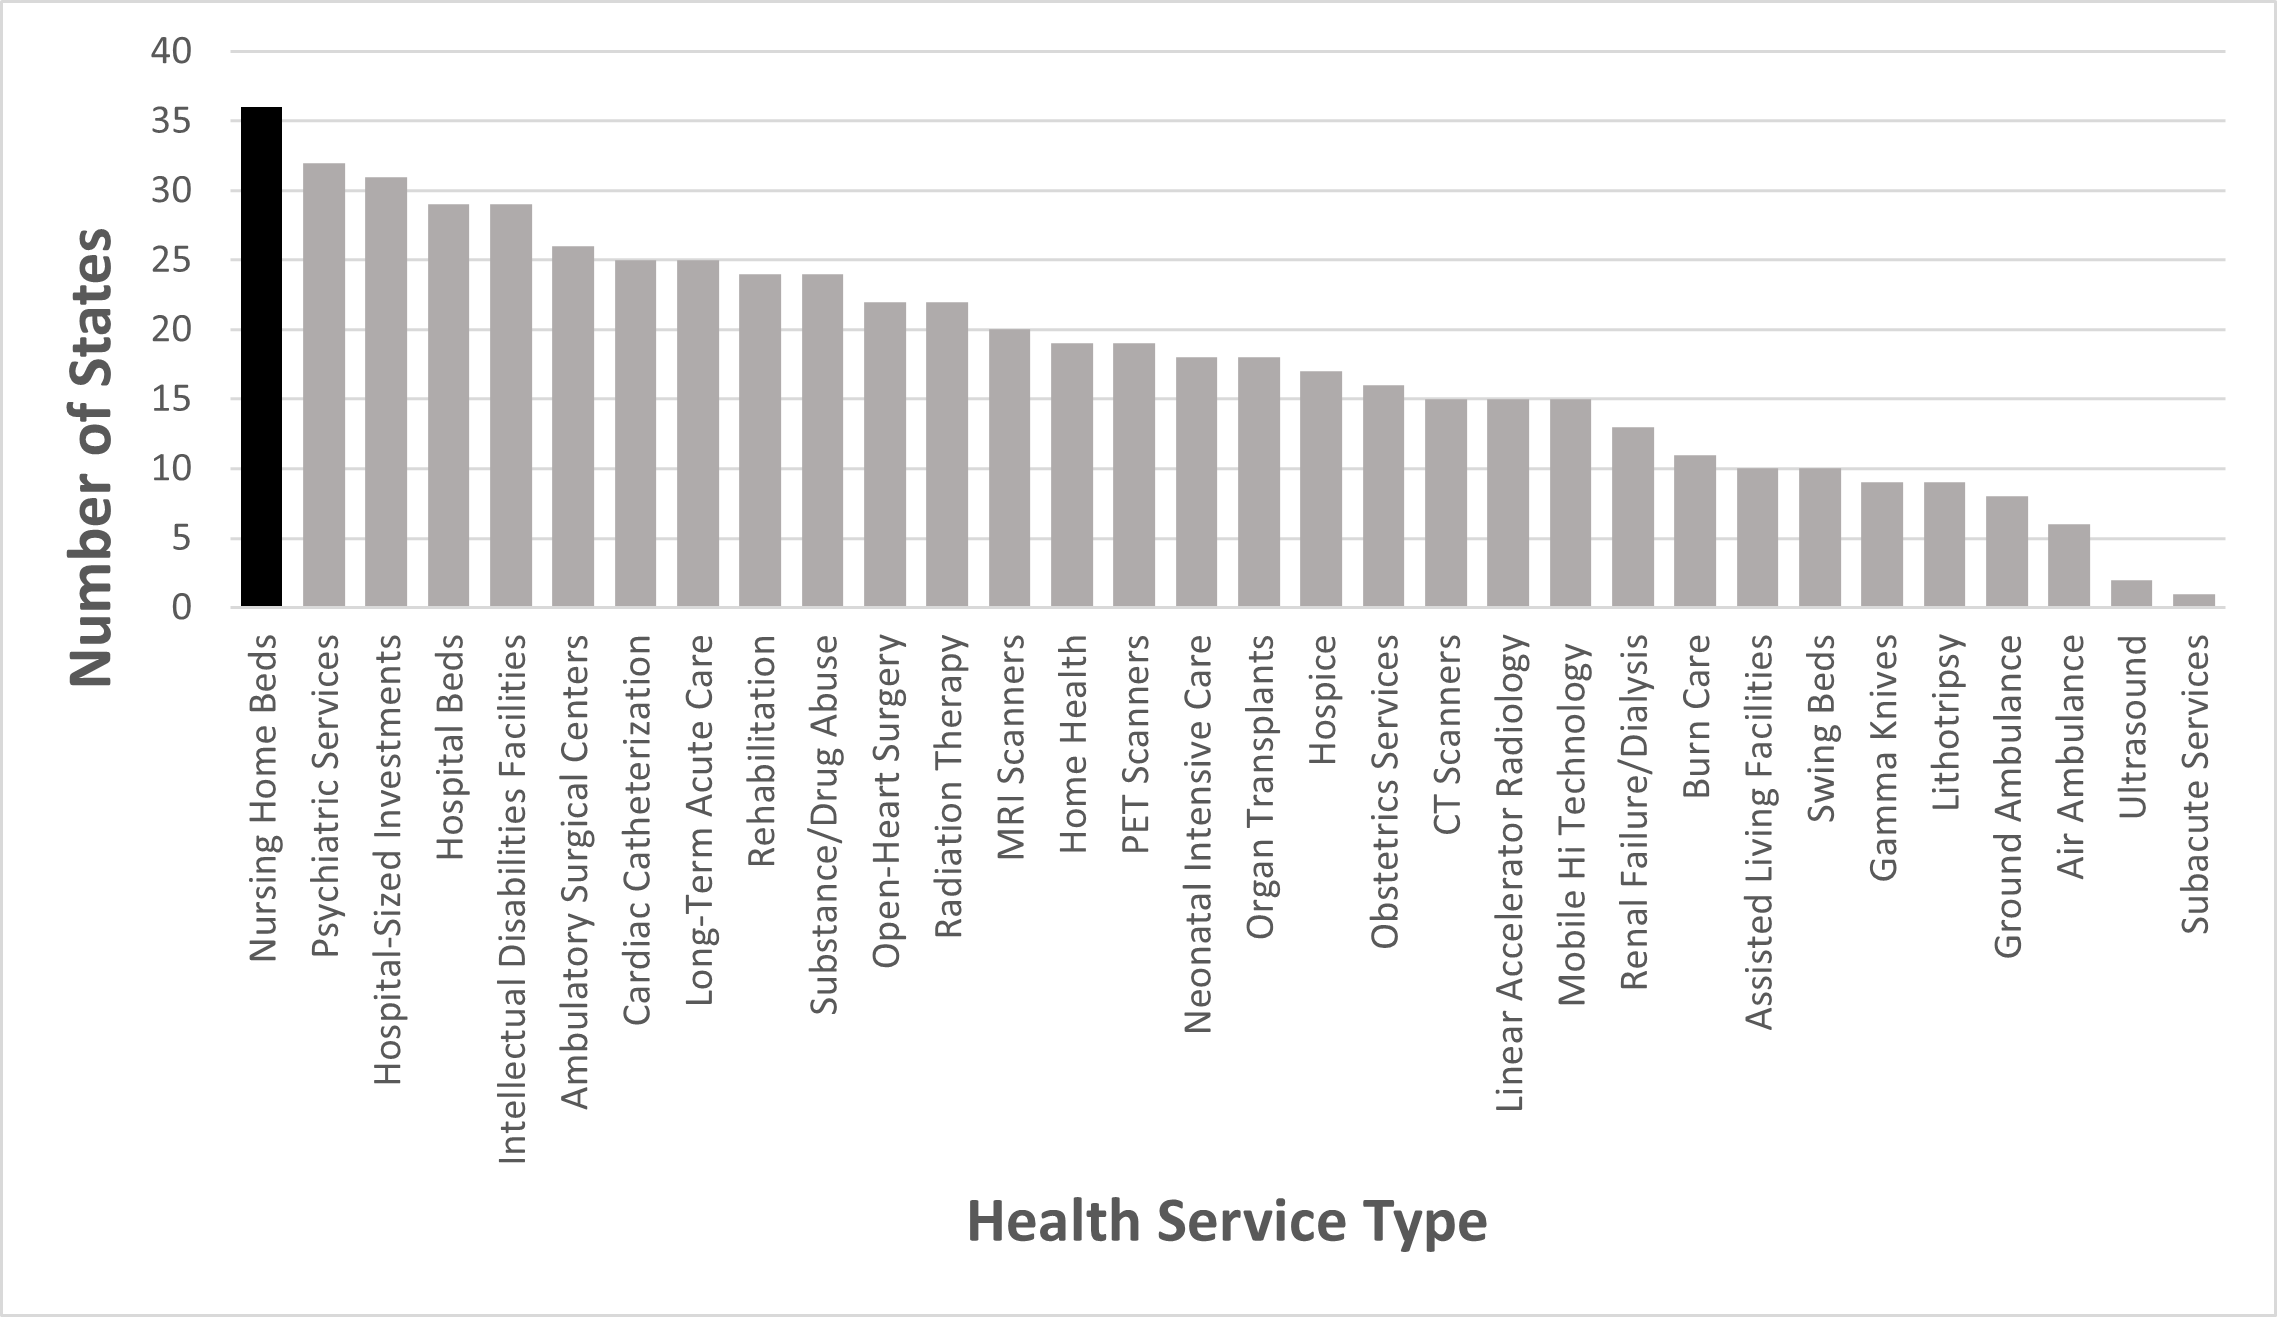
\includegraphics[width=\textwidth,keepaspectratio]{Corrected_Hist.png}
    \end{center}
    \footnotesize
		\textit{Notes}: This figure shows the number of states regulating each health service category in 2020. A total of 36 states regulate nursing home beds, as shown in black. All other services that are regulated by CON are shown in gray. Data source: American Health Planning Association (AHPA).
\end{figure}
\clearpage

\newpage
\begin{figure}[t]
	\begin{center}
	\caption{\label{fig:nh_con_map} \centering Nursing Home Certificate-of-Need Regulation in the United States}
    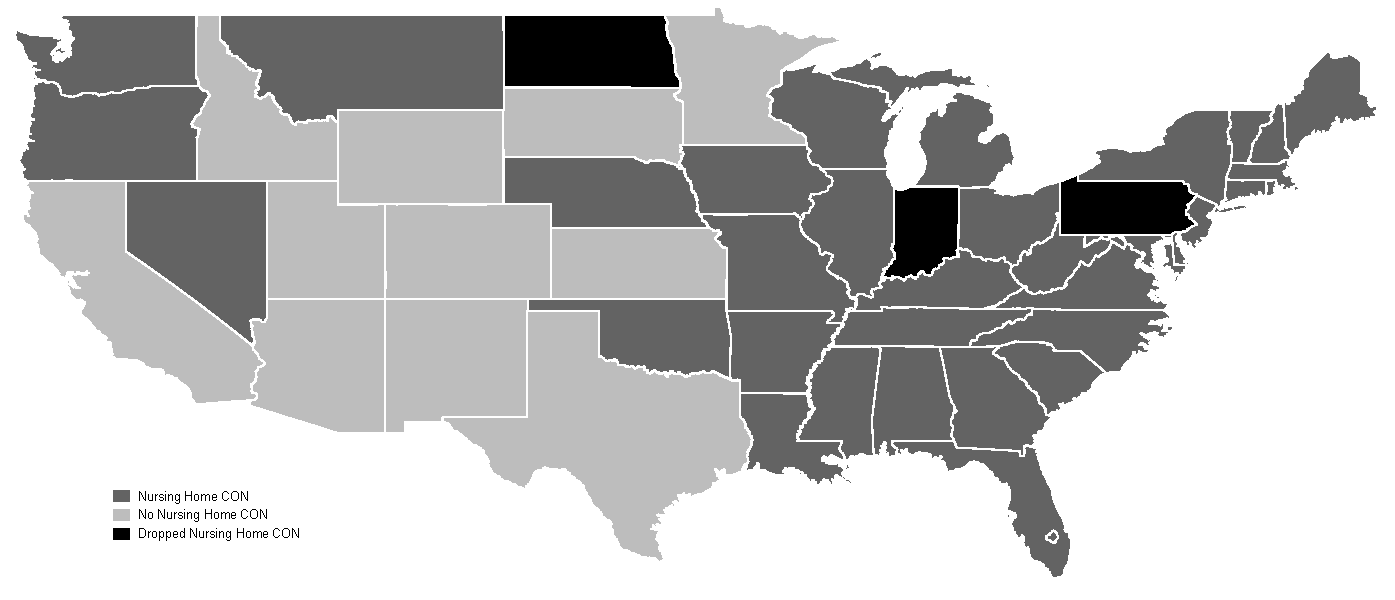
\includegraphics[width=\textwidth,keepaspectratio]{CON_Map.pdf}
    \end{center}
    \footnotesize
		\textit{Notes}: This figure shows which states dropped nursing home CON regulations during our sample period (black), and which states did (dark gray) and did not (light gray) have nursing home CON regulations during our sample period. All of the states that had nursing home CON during our sample period except Connecticut and Louisiana, both of which adopted nursing home CON during the sample period, were included in our donor pool of potential controls when finding synthetic matches for the states that dropped nursing home CON. Data source: American Health Planning Association (AHPA) and the National Conference of State Legislatures.
\end{figure}
\clearpage


\newpage
\begin{figure}[t]
    \begin{center}
	\caption{\label{fig:model_graph} The Effect of Nursing Home CON on Nursing Home Quality}
	\begin{tikzpicture}[scale=1]
    % Axis
    \coordinate (y) at (0,9);
    \coordinate (x) at (10,0);
    \draw[<->] (y) node[above] {$c_z'(z_i)$} -- (0,0) --  (x) node[right] {$z_i$};
    \node [above] at (0,9.6) {$MB(z_i)$,};
    % Draw help grid
    %\draw[step=10mm, lightgray] (0,0) grid (10,10); 
    % define some coordinates
    %\path
    \coordinate (cstart) at (0,0);
    \coordinate (cend) at (10,8);
    \coordinate (mb0start) at (0,1.5);
    \coordinate (mb0end) at (10,6);
    \coordinate (mb1start) at (0,1.2);
    \coordinate (mb1end) at (10,4.5);
    % Draw the lines
     \draw[thick, name path=c] (cstart) to[bend right = 30] (cend) node[right] {$c_z'(z_i)$};
     \draw[thick, name path=mb0] (mb0start) to[bend left = 15] (mb0end) node[right] {$MB^{No~CON}(z_i)$};
     \draw[thick, name path=mb1] (mb1start) to[bend left = 15] (mb1end) node[right] {$MB^{CON}(z_i)$};
     \path[name intersections={of=c and mb0, by=eq0}];
     \draw[black,fill] (eq0) circle[radius = 2pt];
    \draw[thick, dotted] (eq0) -- (eq0 |- 0,0) node[below,xshift=.35cm]{$z_i^{*No~CON}$};
    \path[name intersections={of=c and mb1, by=eq1}];
     \draw[black,fill] (eq1) circle[radius = 2pt];
    \draw[thick, dotted] (eq1) -- (eq1 |- 0,0) node[below,xshift=-.1cm]{$z_i^{*CON}$};
\end{tikzpicture}\\
		\end{center}
		\footnotesize
		\textit{Notes}: This figure shows graphically the effect of implementing nursing home CON regulations on nursing home quality. $MB^{No~CON}(z_i)$ and $MB^{CON}(z_i)$ represent the marginal benefit of increasing quality with and without nursing home CON, and are equal to $\frac{\partial [\prod_{j\neq i} prob(z_i^* -z_j > b_{ji})]}{\partial z_i}(P-c)$ and  $\frac{\partial [\prod_{j\neq i} prob(z_i^* -z_j > b_{ji})]}{\partial z_i}(P-c-R)$, respectively. $c_z'(z_i)=\frac{\partial c_z(z_i^*)}{\partial z_i}$ represents the marginal cost of increasing quality. The implementation of nursing home CON leads to a reduction in the equilibrium nursing home quality. Similarly, the repeal of nursing home CON leads to an increase in the equilibrium nursing home quality.
	\end{figure}
\clearpage


%%%%%%%%%%%%% Medicaid Expenditure Per Capita - PA %%%%%%%%%%%%%
\newpage
\newgeometry{top=2cm}
%\setlength\abovecaptionskip{-1.5\baselineskip}
\begin{figure}[t] 
    \setlength\abovecaptionskip{-2\baselineskip}
	\caption{\label{fig:med_exp_plots_pa} \centering A Comparison Between DID, SC, and SDID Estimates and Placebo Analysis for the Effect of Dropping nursing home CON Regulations on Per Capita Medicaid Nursing Home Expenditure in Pennsylvania} {\centering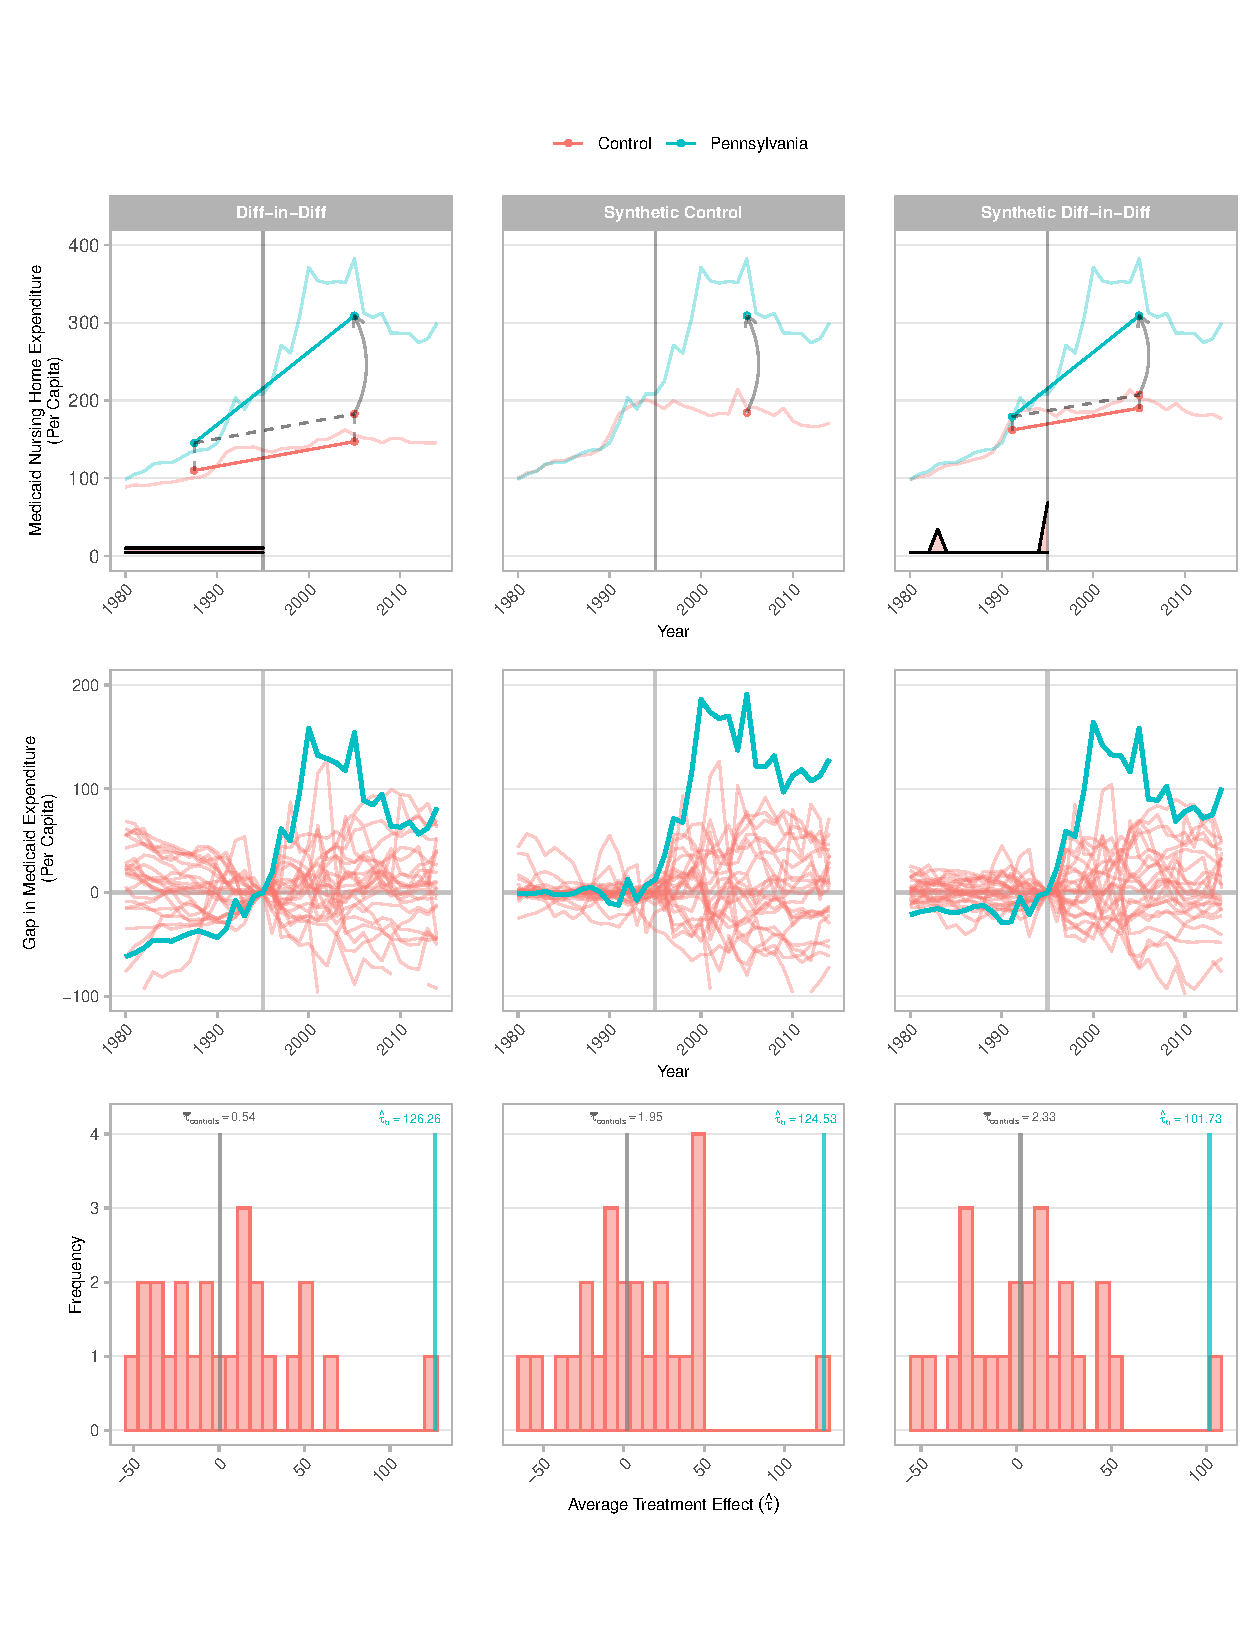
\includegraphics[width=\textwidth,keepaspectratio]{SynthDID_NoBord_NoCov/med_exp_plots_PA.pdf}}
    \vspace{-1.4cm}\\
    \scriptsize
		\textit{Notes}: The plots in the first row show trends in per capita Medicaid nursing home expenditure over time for Pennsylvania and for the relevant weighted average of control states, with the weights used to average pre-treatment time periods at the bottom of the plots. The curved arrows in the first row indicate the estimated average treatment effect, $\hat{\tau}$ from equation (\ref{eq:ave_effect_deltas}), and the vertical lines represent the year prior to PA dropping nursing home CON regulations. The plots in the second row show the year-specific difference in per capita Medicaid nursing home expenditure between PA and its corresponding weighted average of control states. The blue line shows these gaps for PA, and the pink lines show these gaps for each of the placebo control states used in the placebo variance estimation procedure outlined in Algorithm \ref{alg:two}. We make the gaps in the Diff-in-Diff and Synthetic Diff-in-Diff plots relative to their value in the year prior to PA dropping nursing home CON regulations (as indicated by the vertical lines). The plots in the third row show the distribution of placebo estimates ($\hat{\tau}^{(b)}$ from Algorithm \ref{alg:two}), with the mean of the placebo estimates and the actual estimated effect for PA indicated by the gray and blue vertical lines, respectively. Data source: 1980-2014 National Health Expenditure Accounts (NHEA).
\end{figure}
\restoregeometry
\clearpage

%%%%%%%%%%%%% Medicaid Expenditure Per Capita - IN %%%%%%%%%%%%%
\newpage
\newgeometry{top=2cm}
%\setlength\abovecaptionskip{-1.5\baselineskip}
\begin{figure}[t] 
    \setlength\abovecaptionskip{-2\baselineskip}
	\caption{\label{fig:med_exp_plots_in} \centering A Comparison Between DID, SC, and SDID Estimates and Placebo Analysis for the Effect of Dropping Nursing Home CON Regulations on Per Capita Medicaid Nursing Home Expenditure in Indiana} {\centering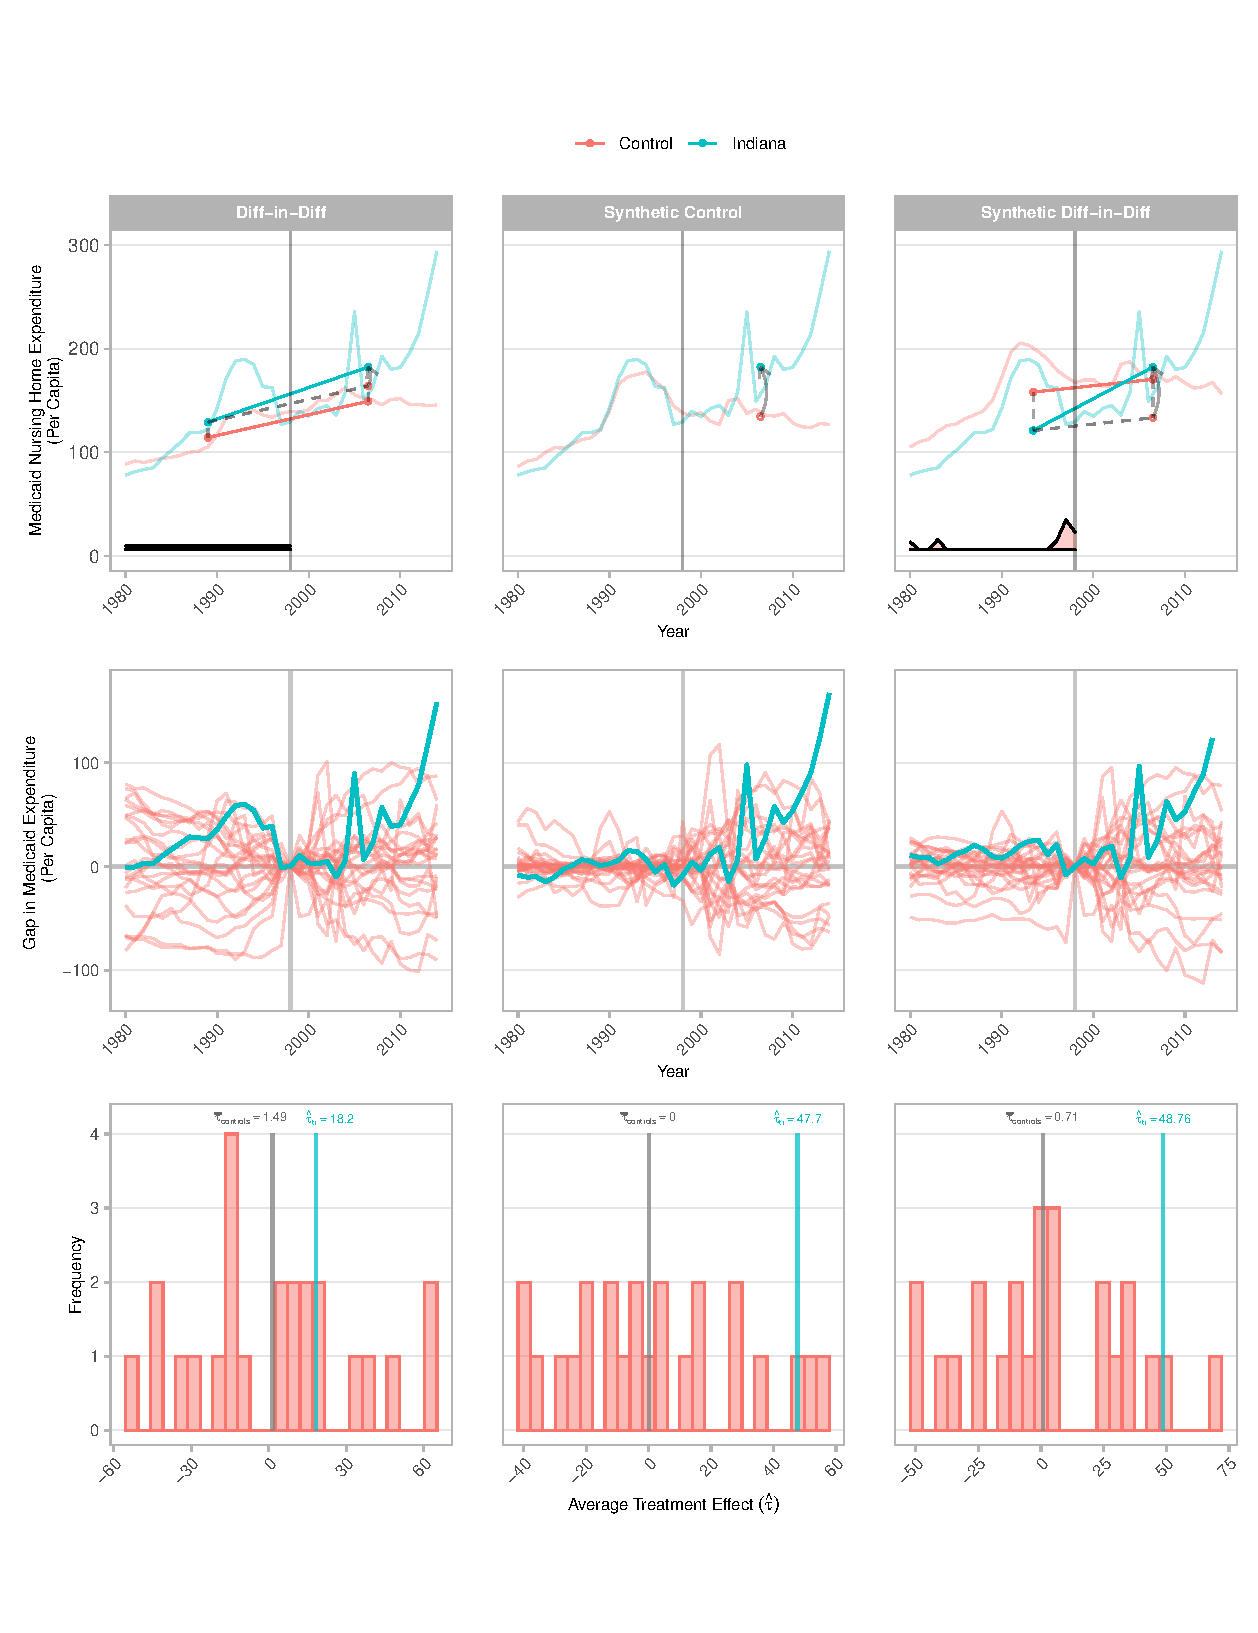
\includegraphics[width=\textwidth,keepaspectratio]{SynthDID_NoBord_NoCov/med_exp_plots_IN.pdf}}
    \vspace{-1.4cm}\\
    \scriptsize
		\textit{Notes}: The plots in the first row show trends in per capita Medicaid nursing home expenditure over time for Indiana and for the relevant weighted average of control states, with the weights used to average pre-treatment time periods at the bottom of the plots. The curved arrows in the first row indicate the estimated average treatment effect, $\hat{\tau}$ from equation (\ref{eq:ave_effect_deltas}), and the vertical lines represent the year prior to IN dropping nursing home CON regulations. The plots in the second row show the year-specific difference in per capita Medicaid nursing home expenditure between IN and its corresponding weighted average of control states. The blue line shows these gaps for IN, and the pink lines show these gaps for each of the placebo control states used in the placebo variance estimation procedure outlined in Algorithm \ref{alg:two}. We make the gaps in the Diff-in-Diff and Synthetic Diff-in-Diff plots relative to their value in the year prior to IN dropping nursing home CON regulations (as indicated by the vertical lines). The plots in the third row show the distribution of placebo estimates ($\hat{\tau}^{(b)}$ from Algorithm \ref{alg:two}), with the mean of the placebo estimates and the actual estimated effect for IN indicated by the gray and blue vertical lines, respectively. Data source: 1980-2014 National Health Expenditure Accounts (NHEA).
\end{figure}
\restoregeometry
\clearpage


%%%%%%%%%%%%% Medicaid Expenditure Per Capita - ND %%%%%%%%%%%%%
\newpage
\newgeometry{top=2cm}
%\setlength\abovecaptionskip{-1.5\baselineskip}
\begin{figure}[t] 
    \setlength\abovecaptionskip{-2\baselineskip}
	\caption{\label{fig:med_exp_plots_nd} \centering A Comparison Between DID, SC, and SDID Estimates and Placebo Analysis for the Effect of Dropping Nursing Home CON Regulations on Per Capita Medicaid Nursing Home Expenditure in North Dakota} {\centering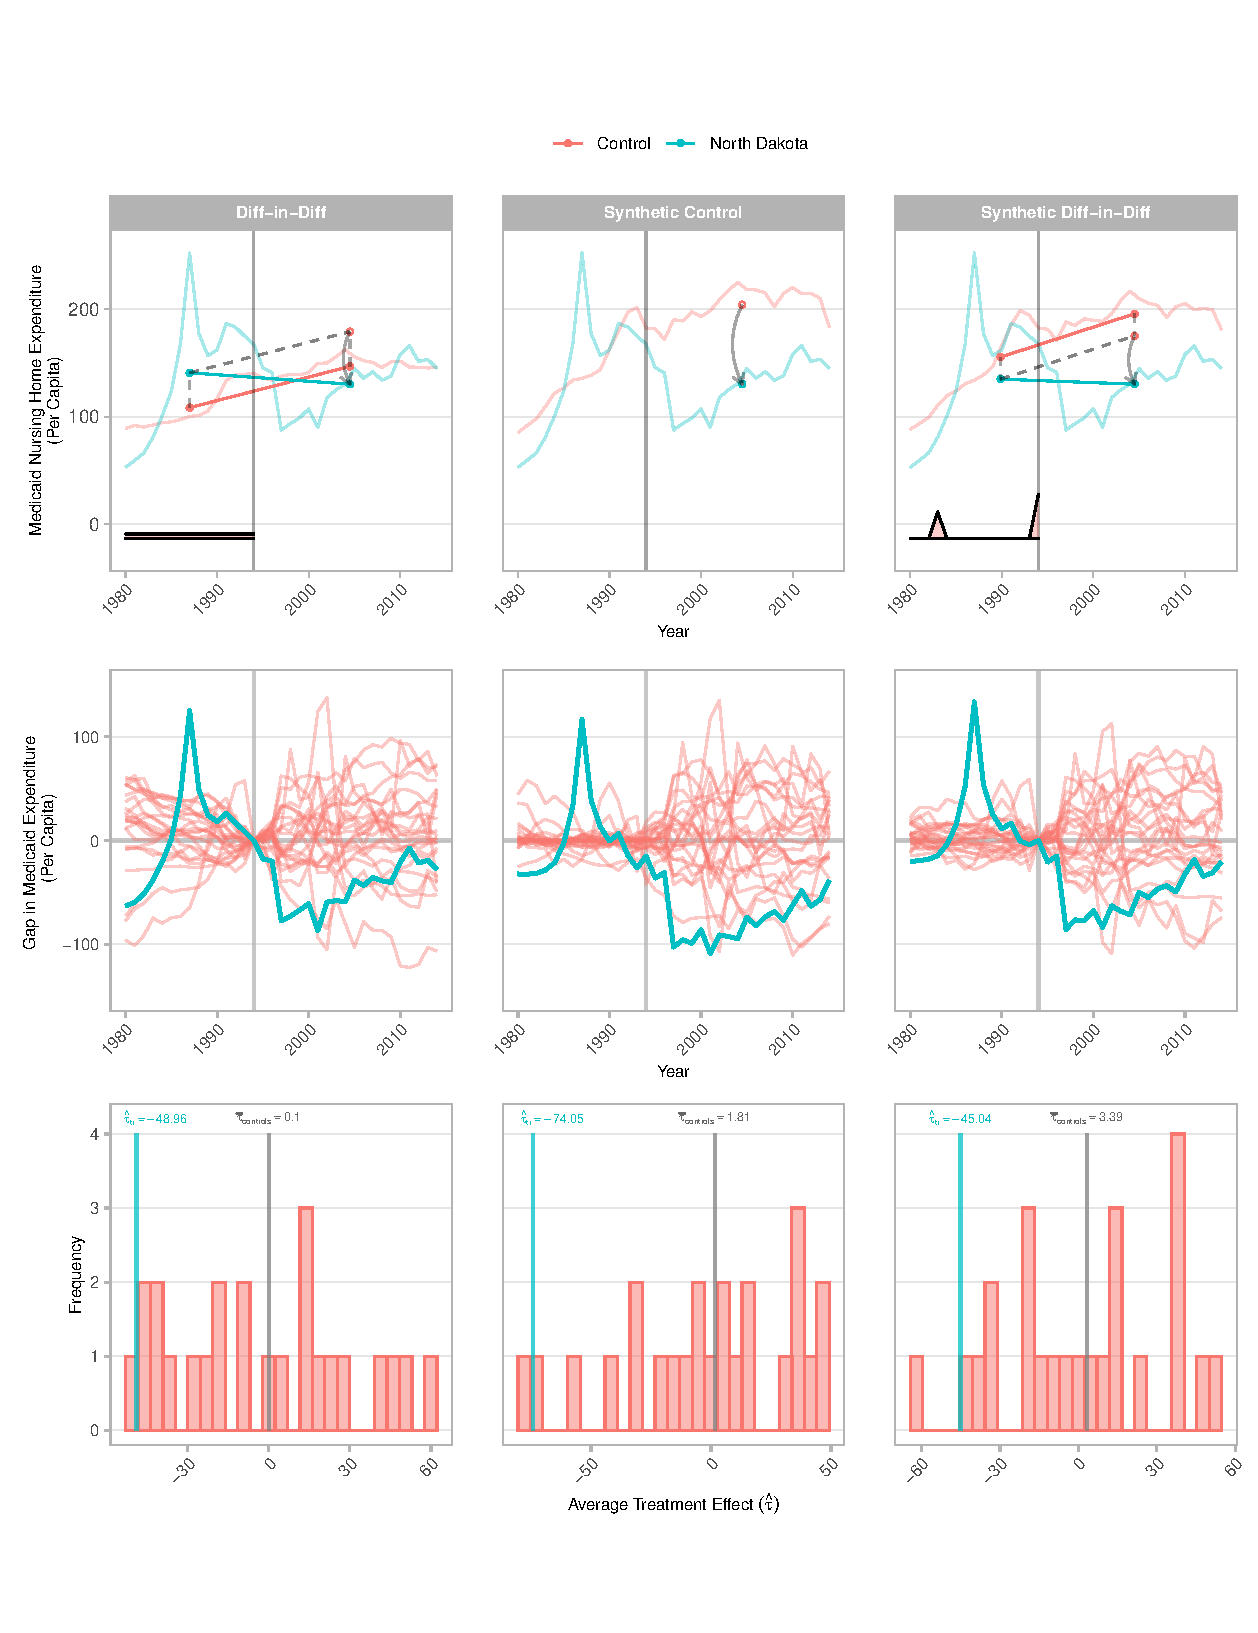
\includegraphics[width=\textwidth,keepaspectratio]{SynthDID_NoBord_NoCov/med_exp_plots_ND.pdf}}
    \vspace{-1.4cm}\\
    \scriptsize
		\textit{Notes}: The plots in the first row show trends in per capita Medicaid nursing home expenditure over time for North Dakota and for the relevant weighted average of control states, with the weights used to average pre-treatment time periods at the bottom of the plots. The curved arrows in the first row indicate the estimated average treatment effect, $\hat{\tau}$ from equation (\ref{eq:ave_effect_deltas}), and the vertical lines represent the year prior to ND dropping nursing home CON regulations. The plots in the second row show the year-specific difference in per capita Medicaid nursing home expenditure between ND and its corresponding weighted average of control states. The blue line shows these gaps for ND, and the pink lines show these gaps for each of the placebo control states used in the placebo variance estimation procedure outlined in Algorithm \ref{alg:two}. We make the gaps in the Diff-in-Diff and Synthetic Diff-in-Diff plots relative to their value in the year prior to ND dropping nursing home CON regulations (as indicated by the vertical lines). The plots in the third row show the distribution of placebo estimates ($\hat{\tau}^{(b)}$ from Algorithm \ref{alg:two}), with the mean of the placebo estimates and the actual estimated effect for ND indicated by the gray and blue vertical lines, respectively. Data source: 1980-2014 National Health Expenditure Accounts (NHEA).
\end{figure}
\restoregeometry
\clearpage


%%%%%%%%%%%%%% Total Expenditure Per Capita - PA %%%%%%%%%%%%%%
\newpage
\newgeometry{top=2cm}
%\setlength\abovecaptionskip{-1.5\baselineskip}
\begin{figure}[t] 
    \setlength\abovecaptionskip{-2\baselineskip}
	\caption{\label{fig:tot_exp_plots_pa} \centering A Comparison Between DID, SC, and SDID Estimates and Placebo Analysis for the Effect of Dropping Nursing Home CON Regulations on Total Per Capita Nursing Home Expenditure in Pennsylvania} {\centering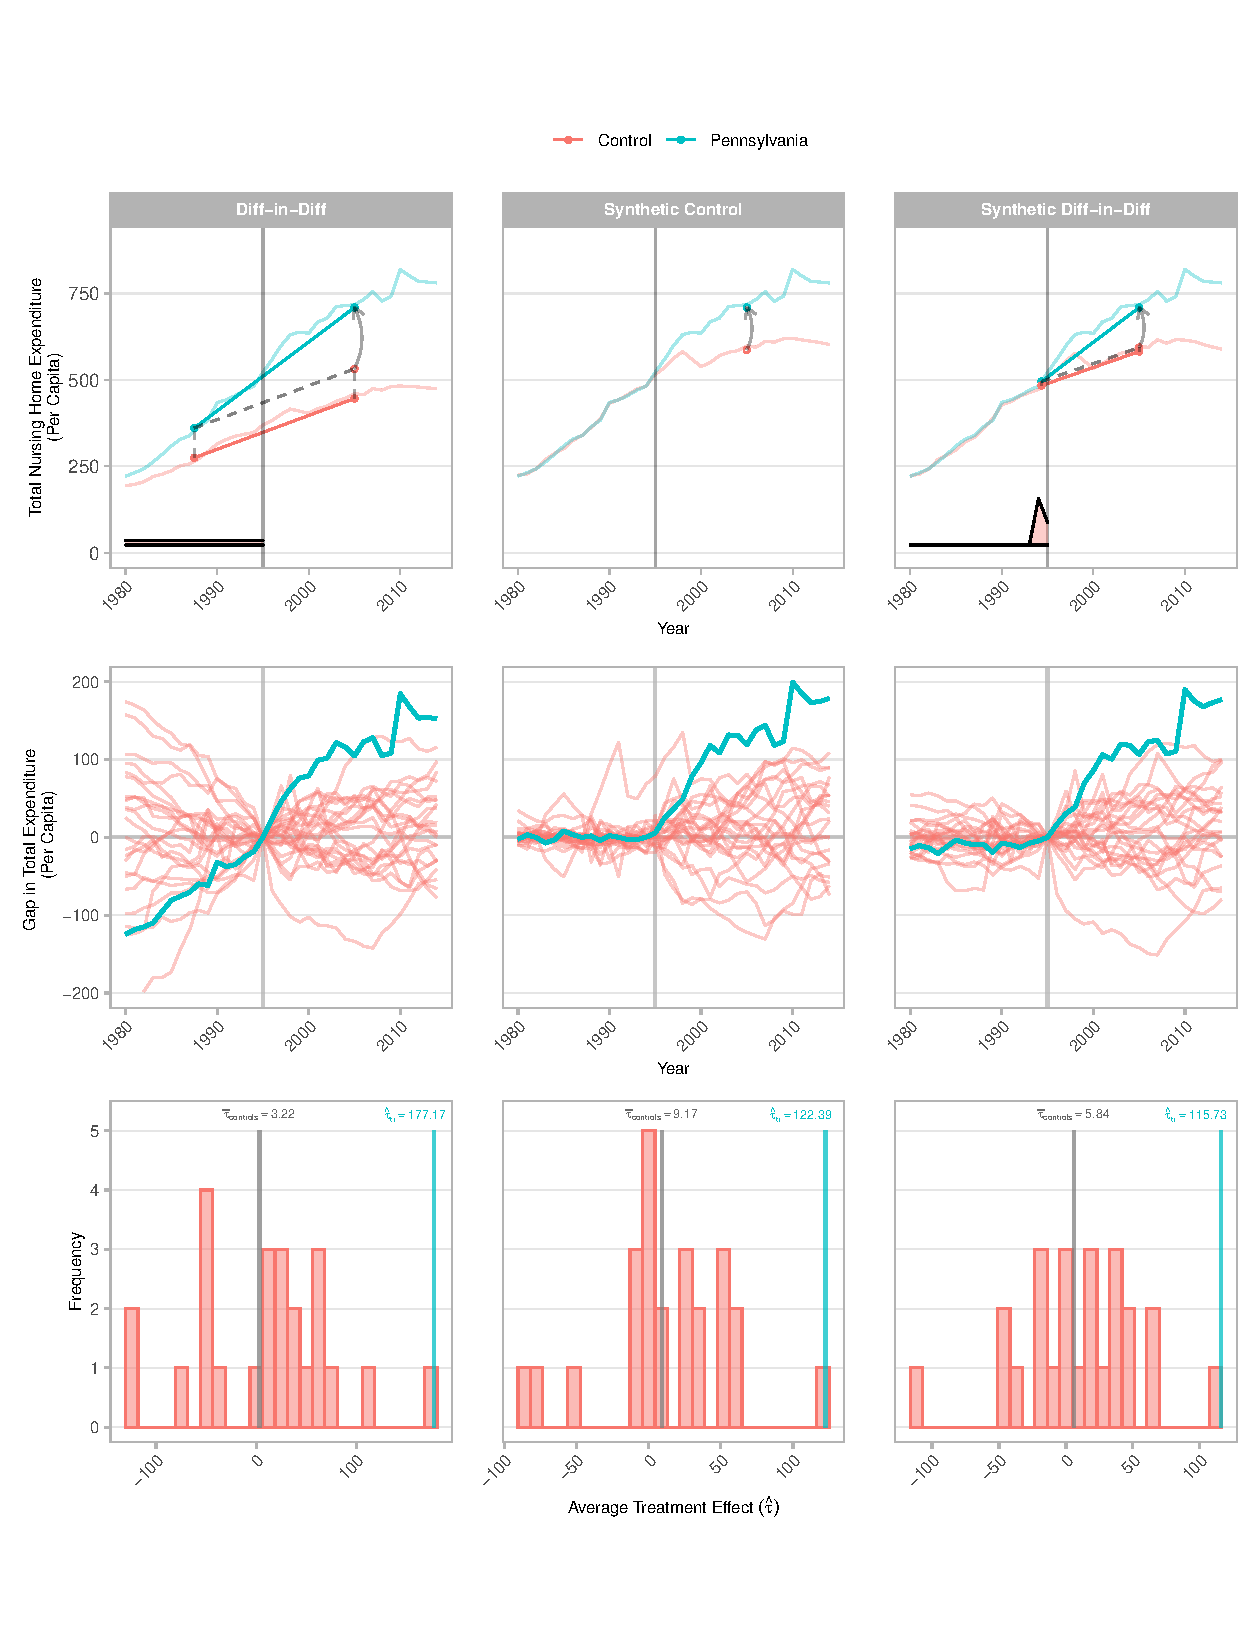
\includegraphics[width=\textwidth,keepaspectratio]{SynthDID_NoBord_NoCov/tot_exp_plots_PA.pdf}}
    \vspace{-1.4cm}\\
    \scriptsize
		\textit{Notes}: The plots in the first row show trends in total per capita nursing home expenditure over time for Pennsylvania and for the relevant weighted average of control states, with the weights used to average pre-treatment time periods at the bottom of the plots. The curved arrows in the first row indicate the estimated average treatment effect, $\hat{\tau}$ from equation (\ref{eq:ave_effect_deltas}), and the vertical lines represent the year prior to PA dropping nursing home CON regulations. The plots in the second row show the year-specific difference in total per capita nursing home expenditure between PA and its corresponding weighted average of control states. The blue line shows these gaps for PA, and the pink lines show these gaps for each of the placebo control states used in the placebo variance estimation procedure outlined in Algorithm \ref{alg:two}. We make the gaps in the Diff-in-Diff and Synthetic Diff-in-Diff plots relative to their value in the year prior to PA dropping nursing home CON regulations (as indicated by the vertical lines). The plots in the third row show the distribution of placebo estimates ($\hat{\tau}^{(b)}$ from Algorithm \ref{alg:two}), with the mean of the placebo estimates and the actual estimated effect for PA indicated by the gray and blue vertical lines, respectively. Data source: 1980-2014 National Health Expenditure Accounts (NHEA).
\end{figure}
\restoregeometry
\clearpage


%%%%%%%%%%%%%% Total Expenditure Per Capita - IN %%%%%%%%%%%%%%
\newpage
\newgeometry{top=2cm}
%\setlength\abovecaptionskip{-1.5\baselineskip}
\begin{figure}[t] 
    \setlength\abovecaptionskip{-2\baselineskip}
	\caption{\label{fig:tot_exp_plots_in} \centering A Comparison Between DID, SC, and SDID Estimates and Placebo Analysis for the Effect of Dropping Nursing Home CON Regulations on Total Per Capita Nursing Home Expenditure in Indiana} {\centering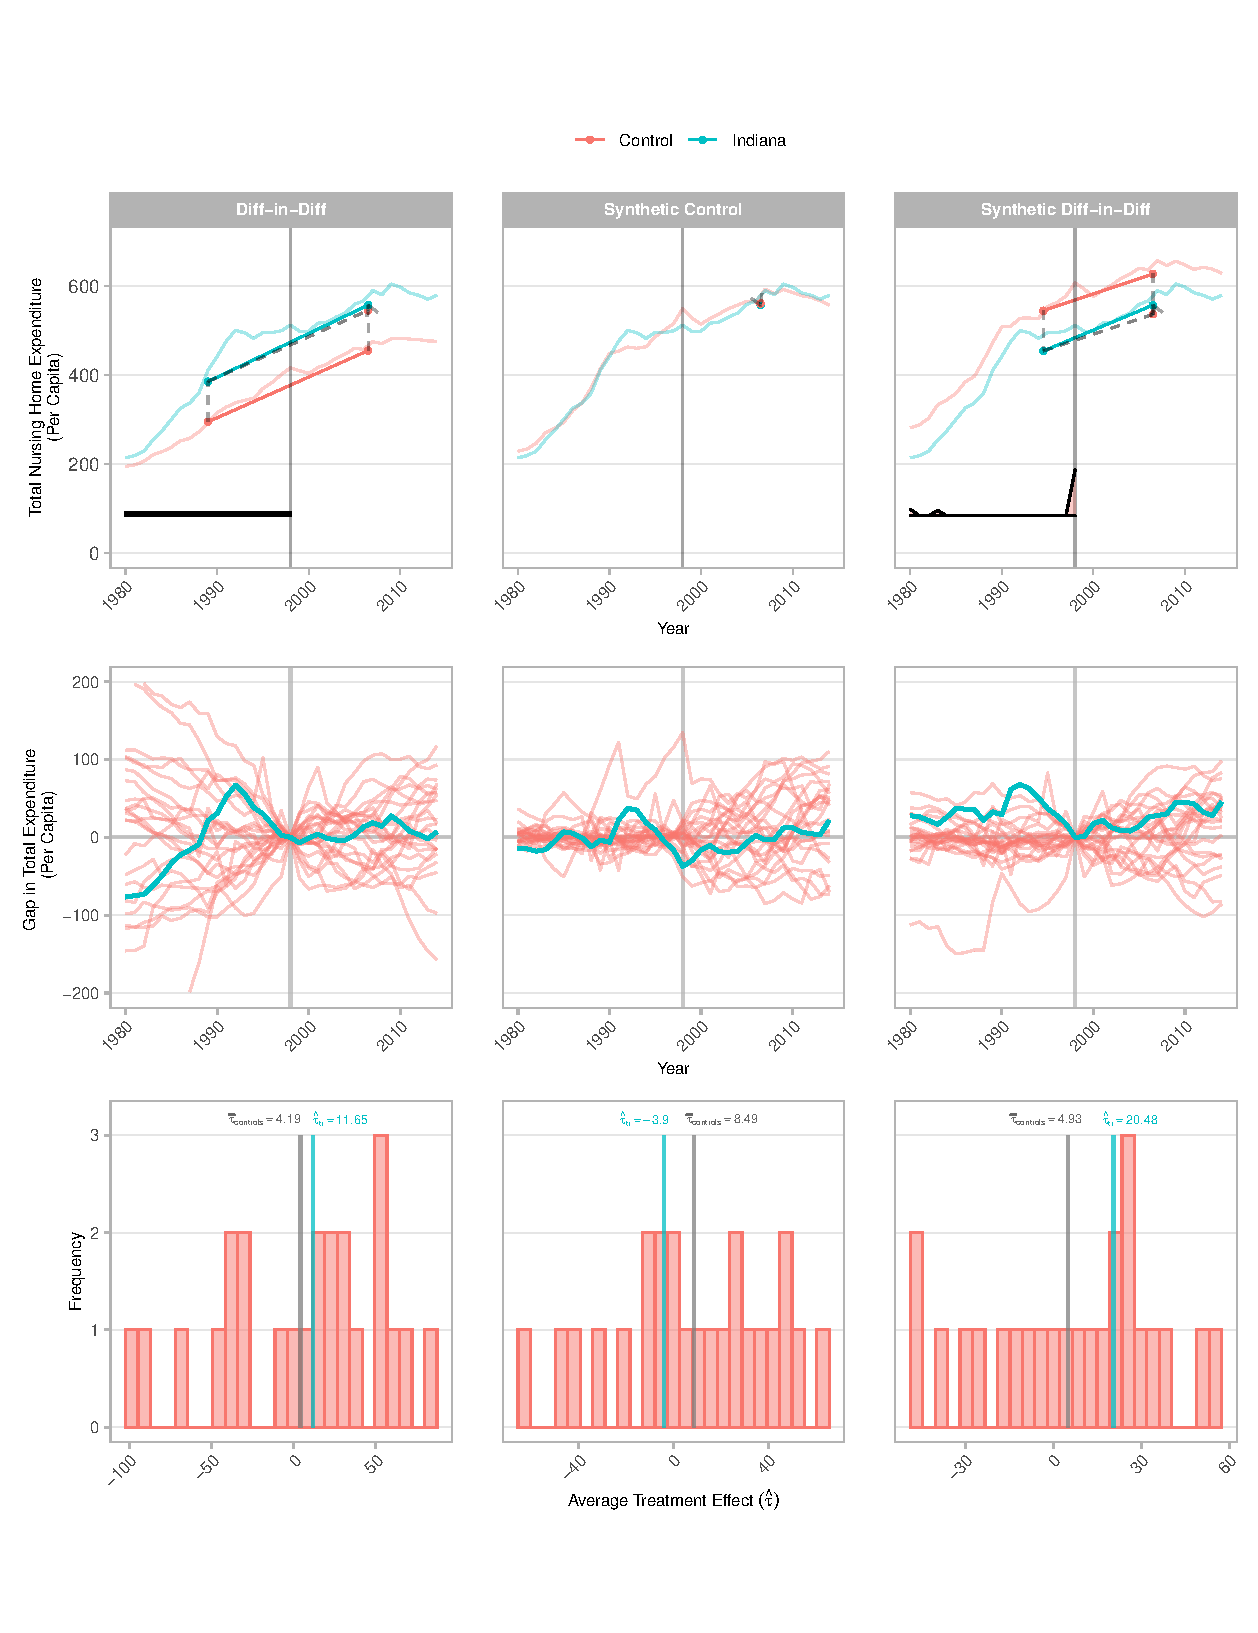
\includegraphics[width=\textwidth,keepaspectratio]{SynthDID_NoBord_NoCov/tot_exp_plots_IN.pdf}}
    \vspace{-1.4cm}\\
    \scriptsize
		\textit{Notes}: The plots in the first row show trends in total per capita nursing home expenditure over time for Indiana and for the relevant weighted average of control states, with the weights used to average pre-treatment time periods at the bottom of the plots. The curved arrows in the first row indicate the estimated average treatment effect, $\hat{\tau}$ from equation (\ref{eq:ave_effect_deltas}), and the vertical lines represent the year prior to IN dropping nursing home CON regulations. The plots in the second row show the year-specific difference in total per capita nursing home expenditure between IN and its corresponding weighted average of control states. The blue line shows these gaps for IN, and the pink lines show these gaps for each of the placebo control states used in the placebo variance estimation procedure outlined in Algorithm \ref{alg:two}. We make the gaps in the Diff-in-Diff and Synthetic Diff-in-Diff plots relative to their value in the year prior to IN dropping nursing home CON regulations (as indicated by the vertical lines). The plots in the third row show the distribution of placebo estimates ($\hat{\tau}^{(b)}$ from Algorithm \ref{alg:two}), with the mean of the placebo estimates and the actual estimated effect for IN indicated by the gray and blue vertical lines, respectively. Data source: 1980-2014 National Health Expenditure Accounts (NHEA).
\end{figure}
\restoregeometry
\clearpage


%%%%%%%%%%%%%% Total Expenditure Per Capita - ND %%%%%%%%%%%%%%
\newpage
\newgeometry{top=2cm}
%\setlength\abovecaptionskip{-1.5\baselineskip}
\begin{figure}[t] 
    \setlength\abovecaptionskip{-2\baselineskip}
	\caption{\label{fig:tot_exp_plots_nd} \centering A Comparison Between DID, SC, and SDID Estimates and Placebo Analysis for the Effect of Dropping Nursing Home CON Regulations on Total Per Capita Nursing Home Expenditure in North Dakota} {\centering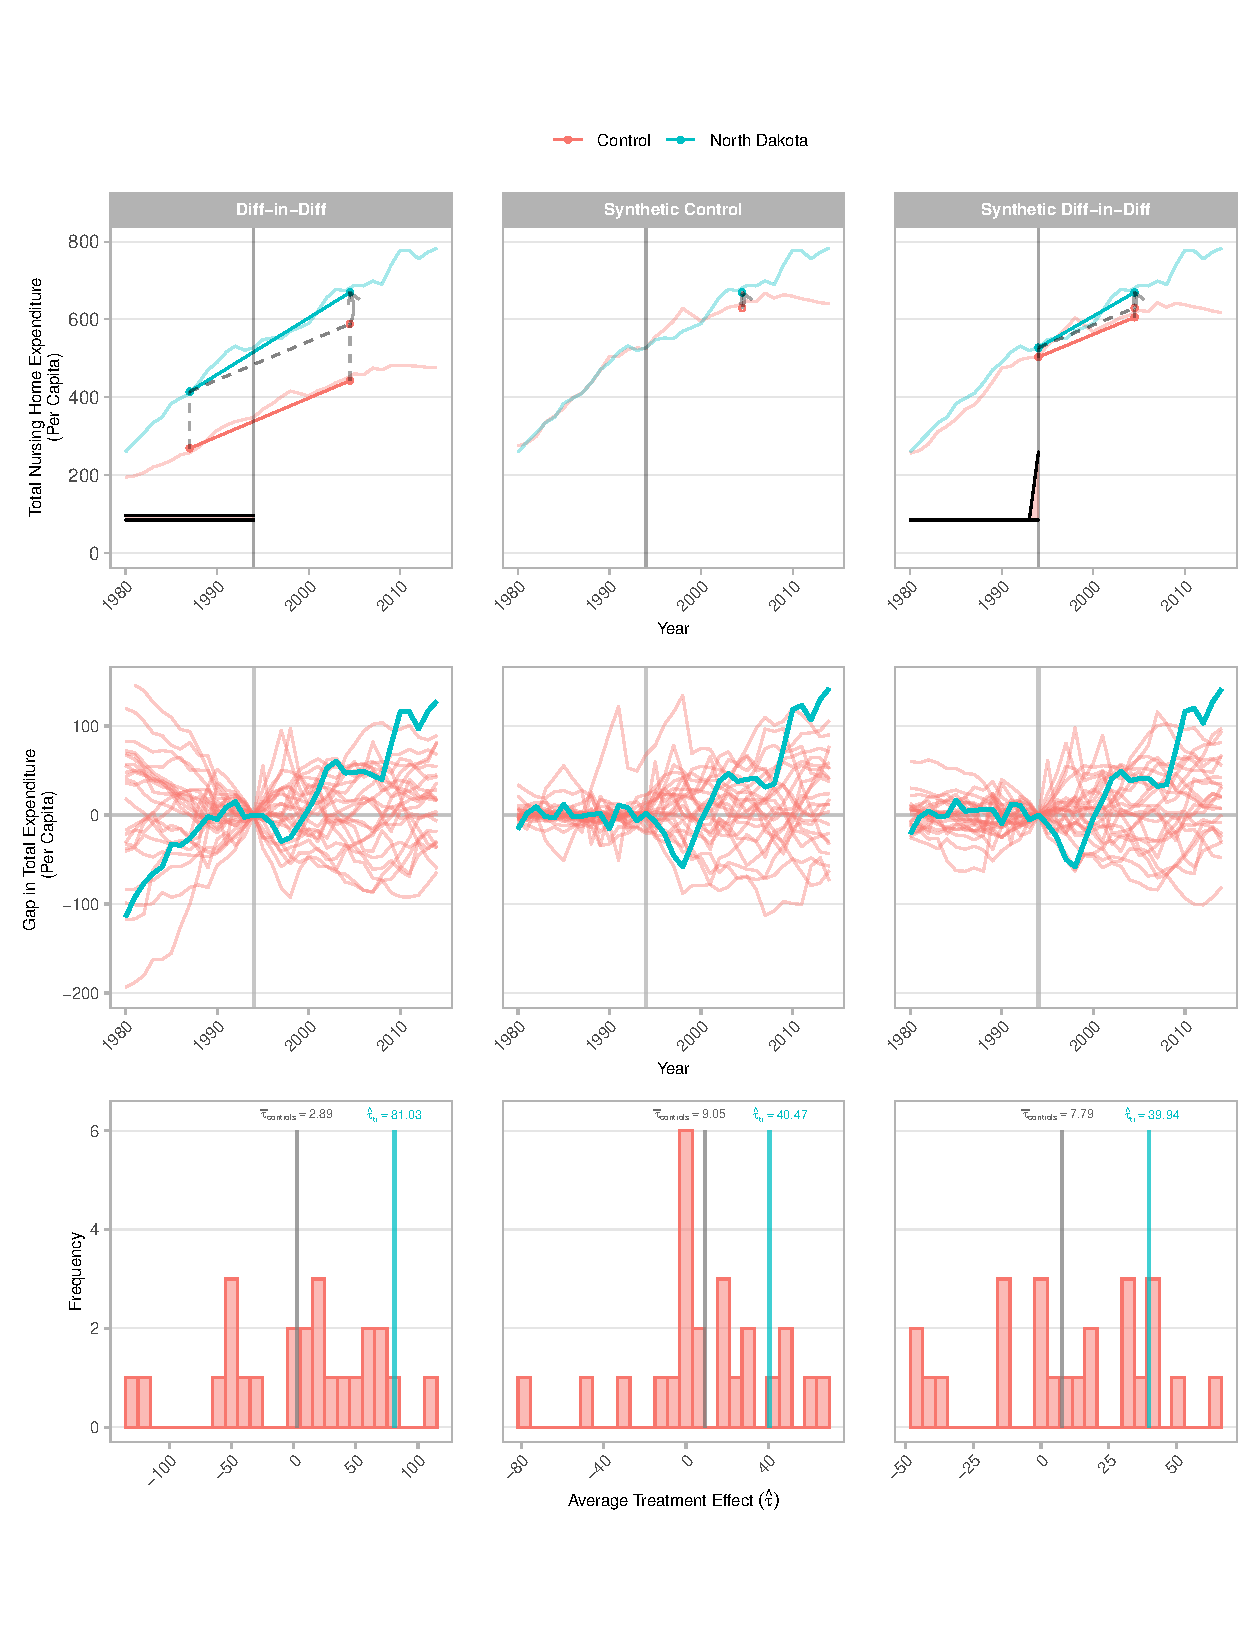
\includegraphics[width=\textwidth,keepaspectratio]{SynthDID_NoBord_NoCov/tot_exp_plots_ND.pdf}}
    \vspace{-1.4cm}\\
    \scriptsize
		\textit{Notes}: The plots in the first row show trends in total per capita nursing home expenditure over time for North Dakota and for the relevant weighted average of control states, with the weights used to average pre-treatment time periods at the bottom of the plots. The curved arrows in the first row indicate the estimated average treatment effect, $\hat{\tau}$ from equation (\ref{eq:ave_effect_deltas}), and the vertical lines represent the year prior to ND dropping nursing home CON regulations. The plots in the second row show the year-specific difference in total per capita nursing home expenditure between ND and its corresponding weighted average of control states. The blue line shows these gaps for ND, and the pink lines show these gaps for each of the placebo control states used in the placebo variance estimation procedure outlined in Algorithm \ref{alg:two}. We make the gaps in the Diff-in-Diff and Synthetic Diff-in-Diff plots relative to their value in the year prior to ND dropping nursing home CON regulations (as indicated by the vertical lines). The plots in the third row show the distribution of placebo estimates ($\hat{\tau}^{(b)}$ from Algorithm \ref{alg:two}), with the mean of the placebo estimates and the actual estimated effect for ND indicated by the gray and blue vertical lines, respectively. Data source: 1980-2014 National Health Expenditure Accounts (NHEA).
\end{figure}
\restoregeometry
\clearpage


%%%%%%%%% Quantity of Certified Beds Per 100,000 - PA %%%%%%%%%%%
\newpage
\newgeometry{top=2cm}
%\setlength\abovecaptionskip{-1.5\baselineskip}
\begin{figure}[t] 
    \setlength\abovecaptionskip{-2\baselineskip}
	\caption{\label{fig:q_certbeds_plots_pa} \centering A Comparison Between DID, SC, and SDID Estimates and Placebo Analysis for the Effect of Dropping Nursing Home CON Regulations on the Quantity of Nursing Home Beds Per 100,000 in Pennsylvania} {\centering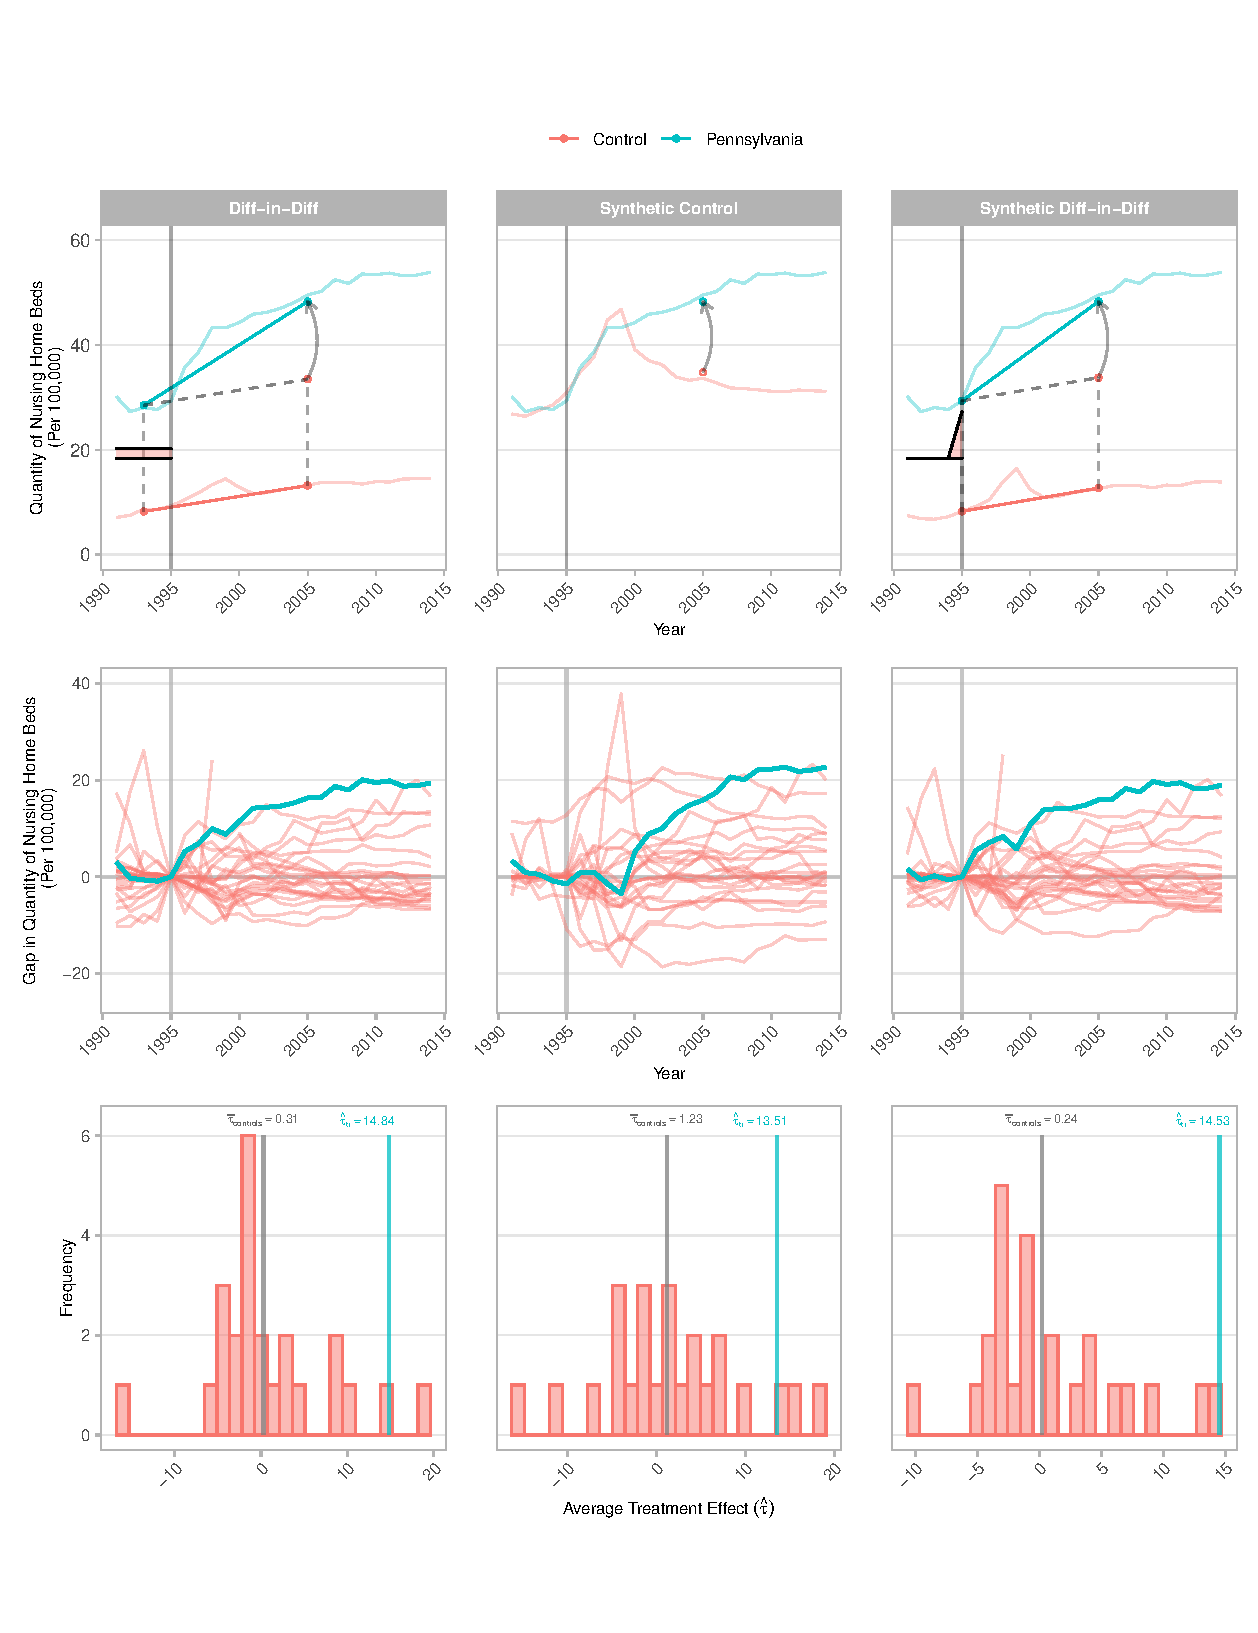
\includegraphics[width=\textwidth,keepaspectratio]{SynthDID_NoBord_NoCov/q_certbeds_plots_PA.pdf}}
    \vspace{-1.4cm}\\
    \scriptsize
		\textit{Notes}: The plots in the first row show trends in the quantity of nursing home beds per 100,000 over time for Pennsylvania and for the relevant weighted average of control states, with the weights used to average pre-treatment time periods at the bottom of the plots. The curved arrows in the first row indicate the estimated average treatment effect, $\hat{\tau}$ from equation (\ref{eq:ave_effect_deltas}), and the vertical lines represent the year prior to PA dropping nursing home CON regulations. The plots in the second row show the year-specific difference in the quantity of nursing home beds per 100,000 between PA and its corresponding weighted average of control states. The blue line shows these gaps for PA, and the pink lines show these gaps for each of the placebo control states used in the placebo variance estimation procedure outlined in Algorithm \ref{alg:two}. We make the gaps in the Diff-in-Diff and Synthetic Diff-in-Diff plots relative to their value in the year prior to PA dropping nursing home CON regulations (as indicated by the vertical lines). The plots in the third row show the distribution of placebo estimates ($\hat{\tau}^{(b)}$ from Algorithm \ref{alg:two}), with the mean of the placebo estimates and the actual estimated effect for PA indicated by the gray and blue vertical lines, respectively. Data source: 1991-2014 Centers for Medicare and Medicaid Services’ (CMS) Provider of Services files.
\end{figure}
\restoregeometry
\clearpage


%%%%%%%%% Quantity of Certified Beds Per 100,000 - IN %%%%%%%%%%%
\newpage
\newgeometry{top=2cm}
%\setlength\abovecaptionskip{-1.5\baselineskip}
\begin{figure}[t] 
    \setlength\abovecaptionskip{-2\baselineskip}
	\caption{\label{fig:q_certbeds_plots_in} \centering A Comparison Between DID, SC, and SDID Estimates and Placebo Analysis for the Effect of Dropping Nursing Home CON Regulations on the Quantity of Nursing Home Beds Per 100,000 in Indiana} {\centering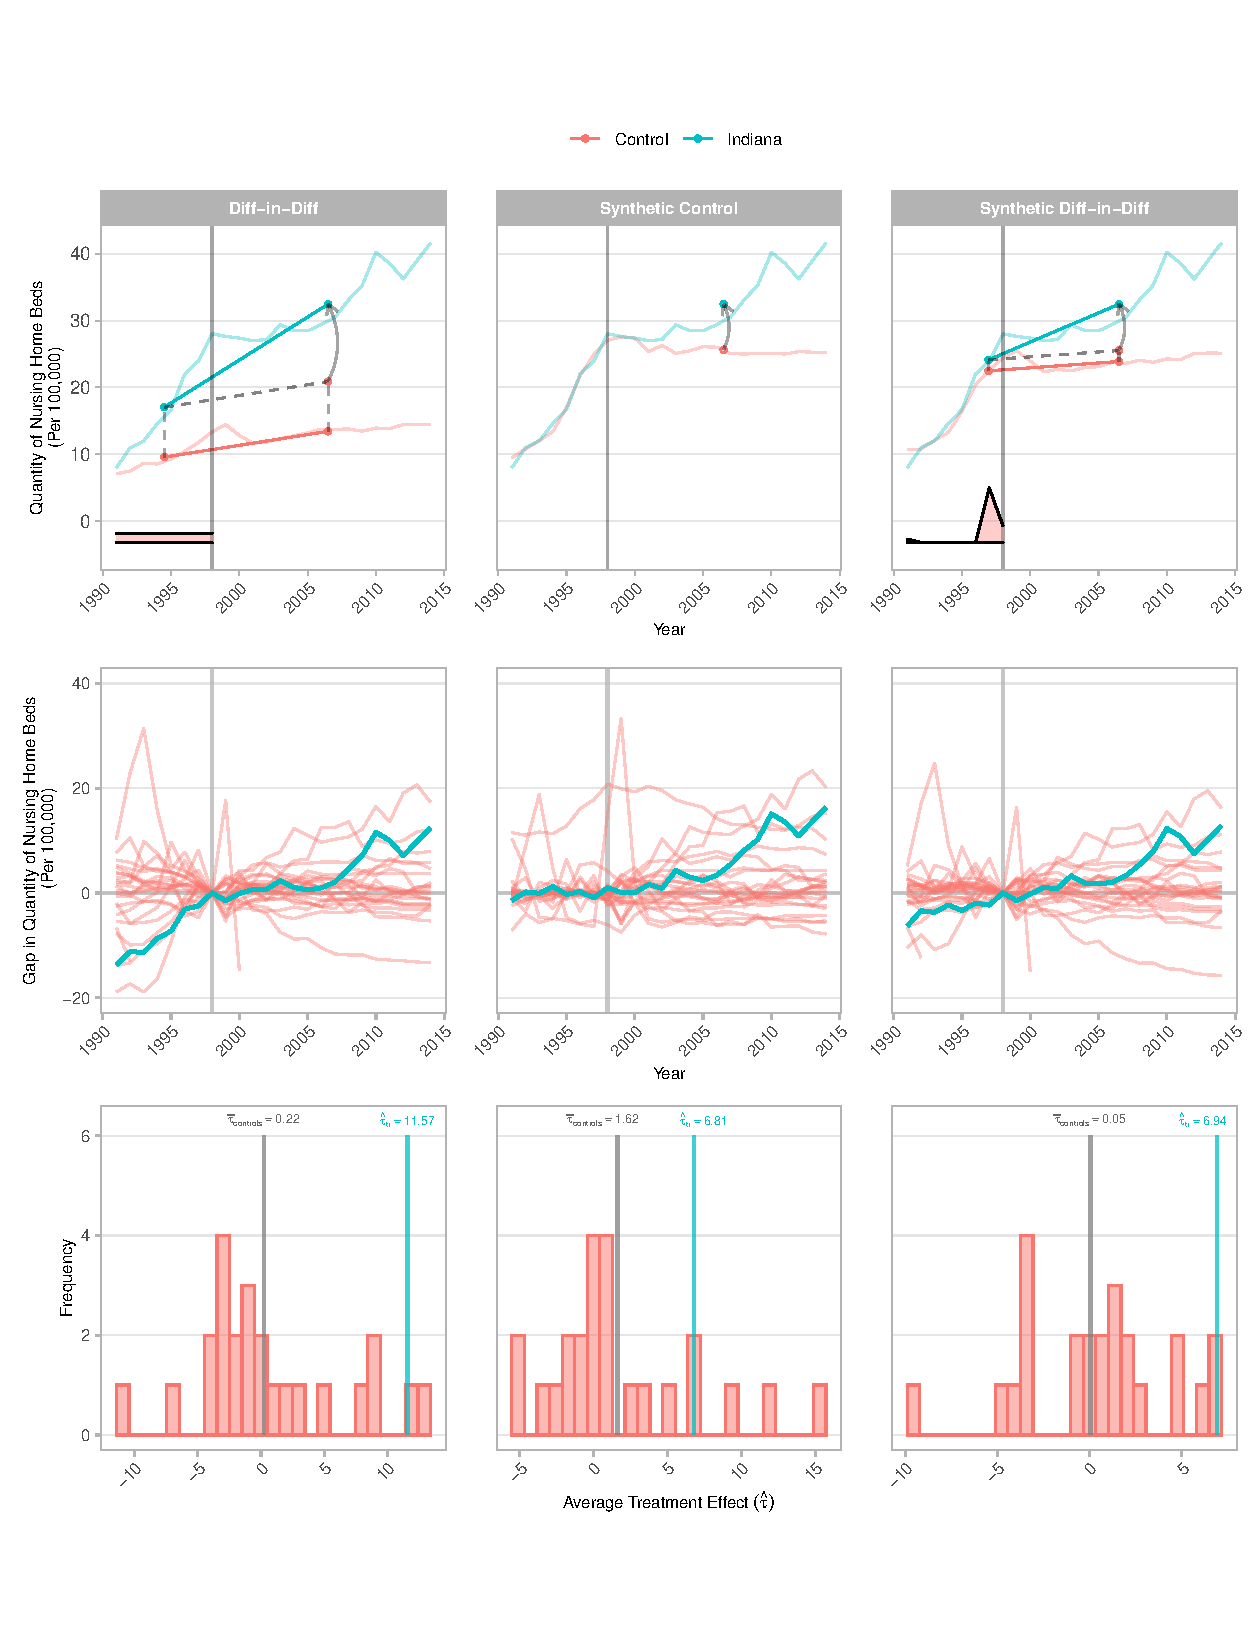
\includegraphics[width=\textwidth,keepaspectratio]{SynthDID_NoBord_NoCov/q_certbeds_plots_IN.pdf}}
    \vspace{-1.4cm}\\
    \scriptsize
		\textit{Notes}: The plots in the first row show trends in the quantity of nursing home beds per 100,000 over time for Indiana and for the relevant weighted average of control states, with the weights used to average pre-treatment time periods at the bottom of the plots. The curved arrows in the first row indicate the estimated average treatment effect, $\hat{\tau}$ from equation (\ref{eq:ave_effect_deltas}), and the vertical lines represent the year prior to IN dropping nursing home CON regulations. The plots in the second row show the year-specific difference in the quantity of nursing home beds per 100,000 between IN and its corresponding weighted average of control states. The blue line shows these gaps for IN, and the pink lines show these gaps for each of the placebo control states used in the placebo variance estimation procedure outlined in Algorithm \ref{alg:two}. We make the gaps in the Diff-in-Diff and Synthetic Diff-in-Diff plots relative to their value in the year prior to IN dropping nursing home CON regulations (as indicated by the vertical lines). The plots in the third row show the distribution of placebo estimates ($\hat{\tau}^{(b)}$ from Algorithm \ref{alg:two}), with the mean of the placebo estimates and the actual estimated effect for IN indicated by the gray and blue vertical lines, respectively. Data source: 1991-2014 Centers for Medicare and Medicaid Services’ (CMS) Provider of Services files.
\end{figure}
\restoregeometry
\clearpage


%%%%%%%%% Quantity of Certified Beds Per 100,000 - ND %%%%%%%%%%%
\newpage
\newgeometry{top=2cm}
%\setlength\abovecaptionskip{-1.5\baselineskip}
\begin{figure}[t] 
    \setlength\abovecaptionskip{-2\baselineskip}
	\caption{\label{fig:q_certbeds_plots_nd} \centering A Comparison Between DID, SC, and SDID Estimates and Placebo Analysis for the Effect of Dropping Nursing Home CON Regulations on the Quantity of Nursing Home Beds Per 100,000 in North Dakota} {\centering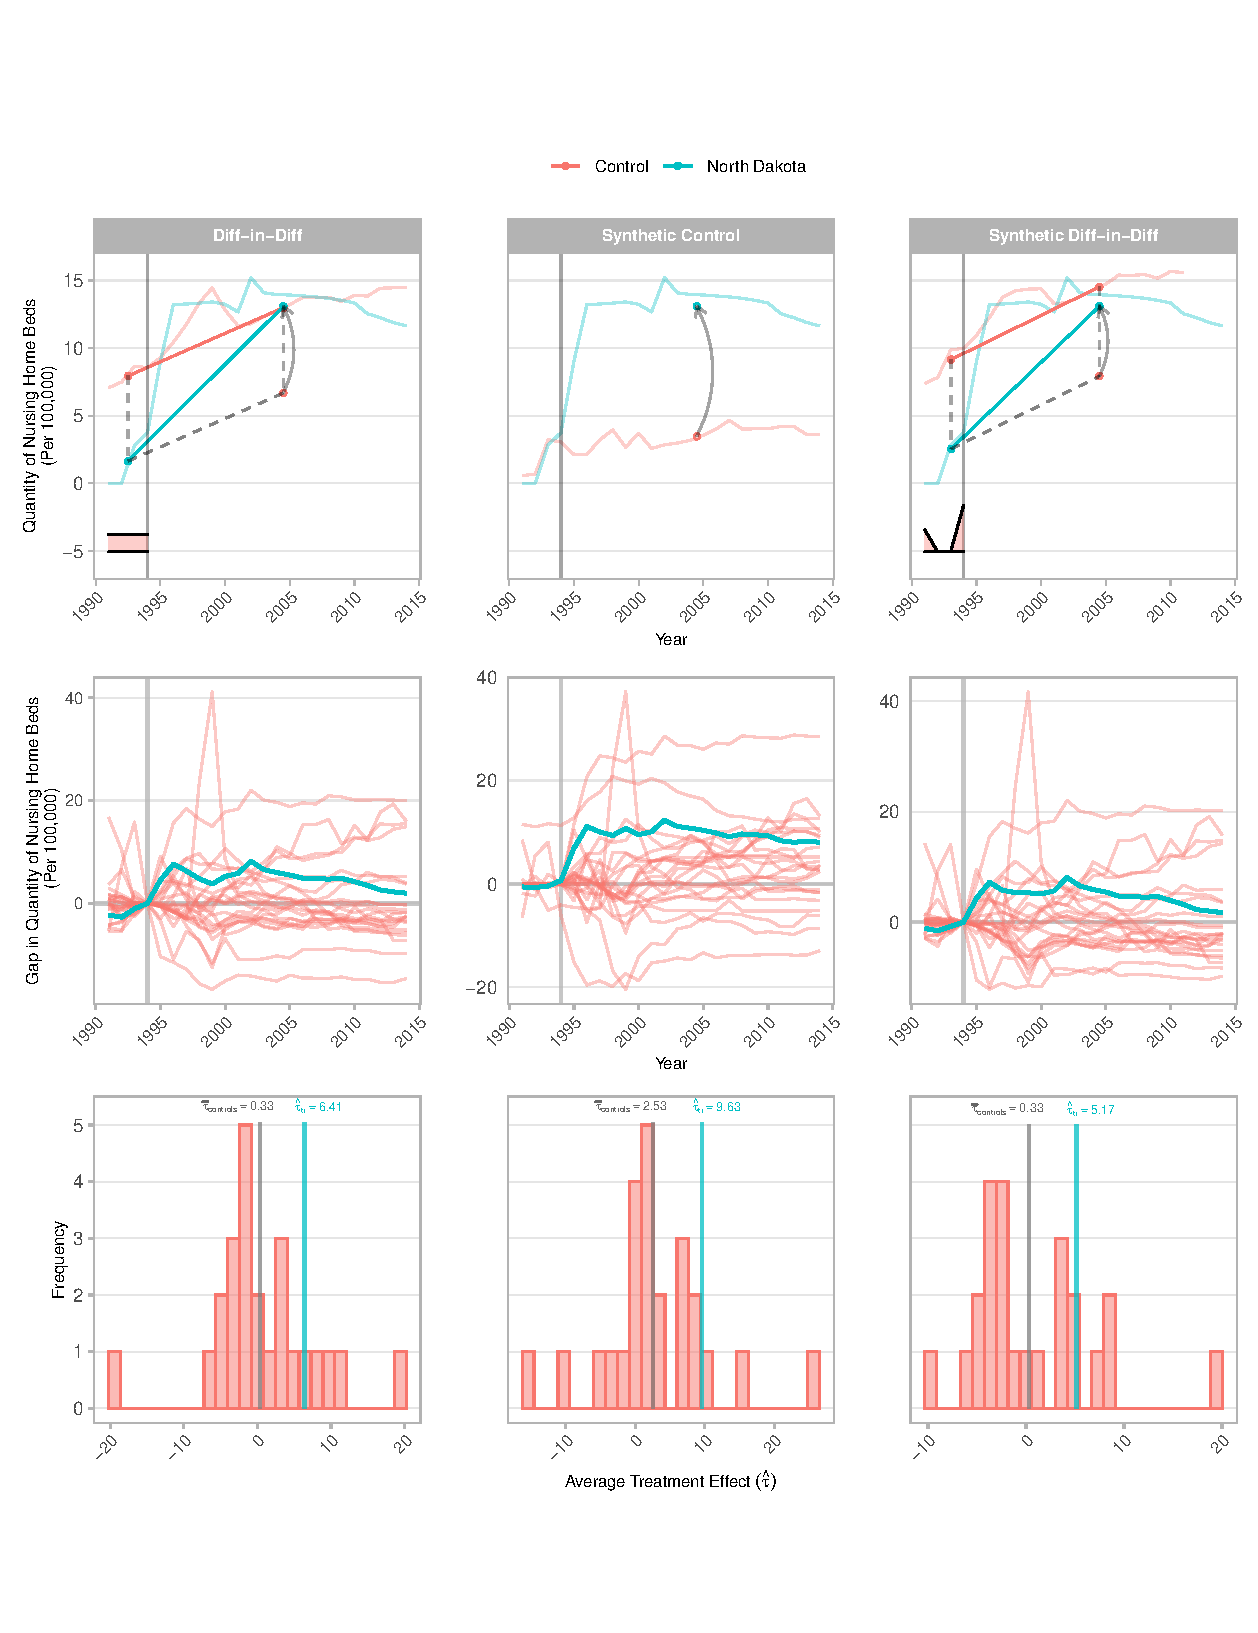
\includegraphics[width=\textwidth,keepaspectratio]{SynthDID_NoBord_NoCov/q_certbeds_plots_ND.pdf}}
    \vspace{-1.4cm}\\
    \scriptsize
		\textit{Notes}: The plots in the first row show trends in the quantity of nursing home beds per 100,000 over time for North Dakota and for the relevant weighted average of control states, with the weights used to average pre-treatment time periods at the bottom of the plots. The curved arrows in the first row indicate the estimated average treatment effect, $\hat{\tau}$ from equation (\ref{eq:ave_effect_deltas}), and the vertical lines represent the year prior to ND dropping nursing home CON regulations. The plots in the second row show the year-specific difference in the quantity of nursing home beds per 100,000 between ND and its corresponding weighted average of control states. The blue line shows these gaps for ND, and the pink lines show these gaps for each of the placebo control states used in the placebo variance estimation procedure outlined in Algorithm \ref{alg:two}. We make the gaps in the Diff-in-Diff and Synthetic Diff-in-Diff plots relative to their value in the year prior to ND dropping nursing home CON regulations (as indicated by the vertical lines). The plots in the third row show the distribution of placebo estimates ($\hat{\tau}^{(b)}$ from Algorithm \ref{alg:two}), with the mean of the placebo estimates and the actual estimated effect for ND indicated by the gray and blue vertical lines, respectively. Data source: 1991-2014 Centers for Medicare and Medicaid Services’ (CMS) Provider of Services files.
\end{figure}
\restoregeometry
\clearpage


%%%%%%%%%%% Quantity of Nursing Homes Per Capita - PA %%%%%%%%%%%
\newpage
\newgeometry{top=2cm}
%\setlength\abovecaptionskip{-1.5\baselineskip}
\begin{figure}[t] 
    \setlength\abovecaptionskip{-2\baselineskip}
	\caption{\label{fig:q_nh_plots_pa} \centering A Comparison Between DID, SC, and SDID Estimates and Placebo Analysis for the Effect of Dropping Nursing Home CON Regulations on the Quantity of Nursing Homes Per 100,000 in Pennsylvania} {\centering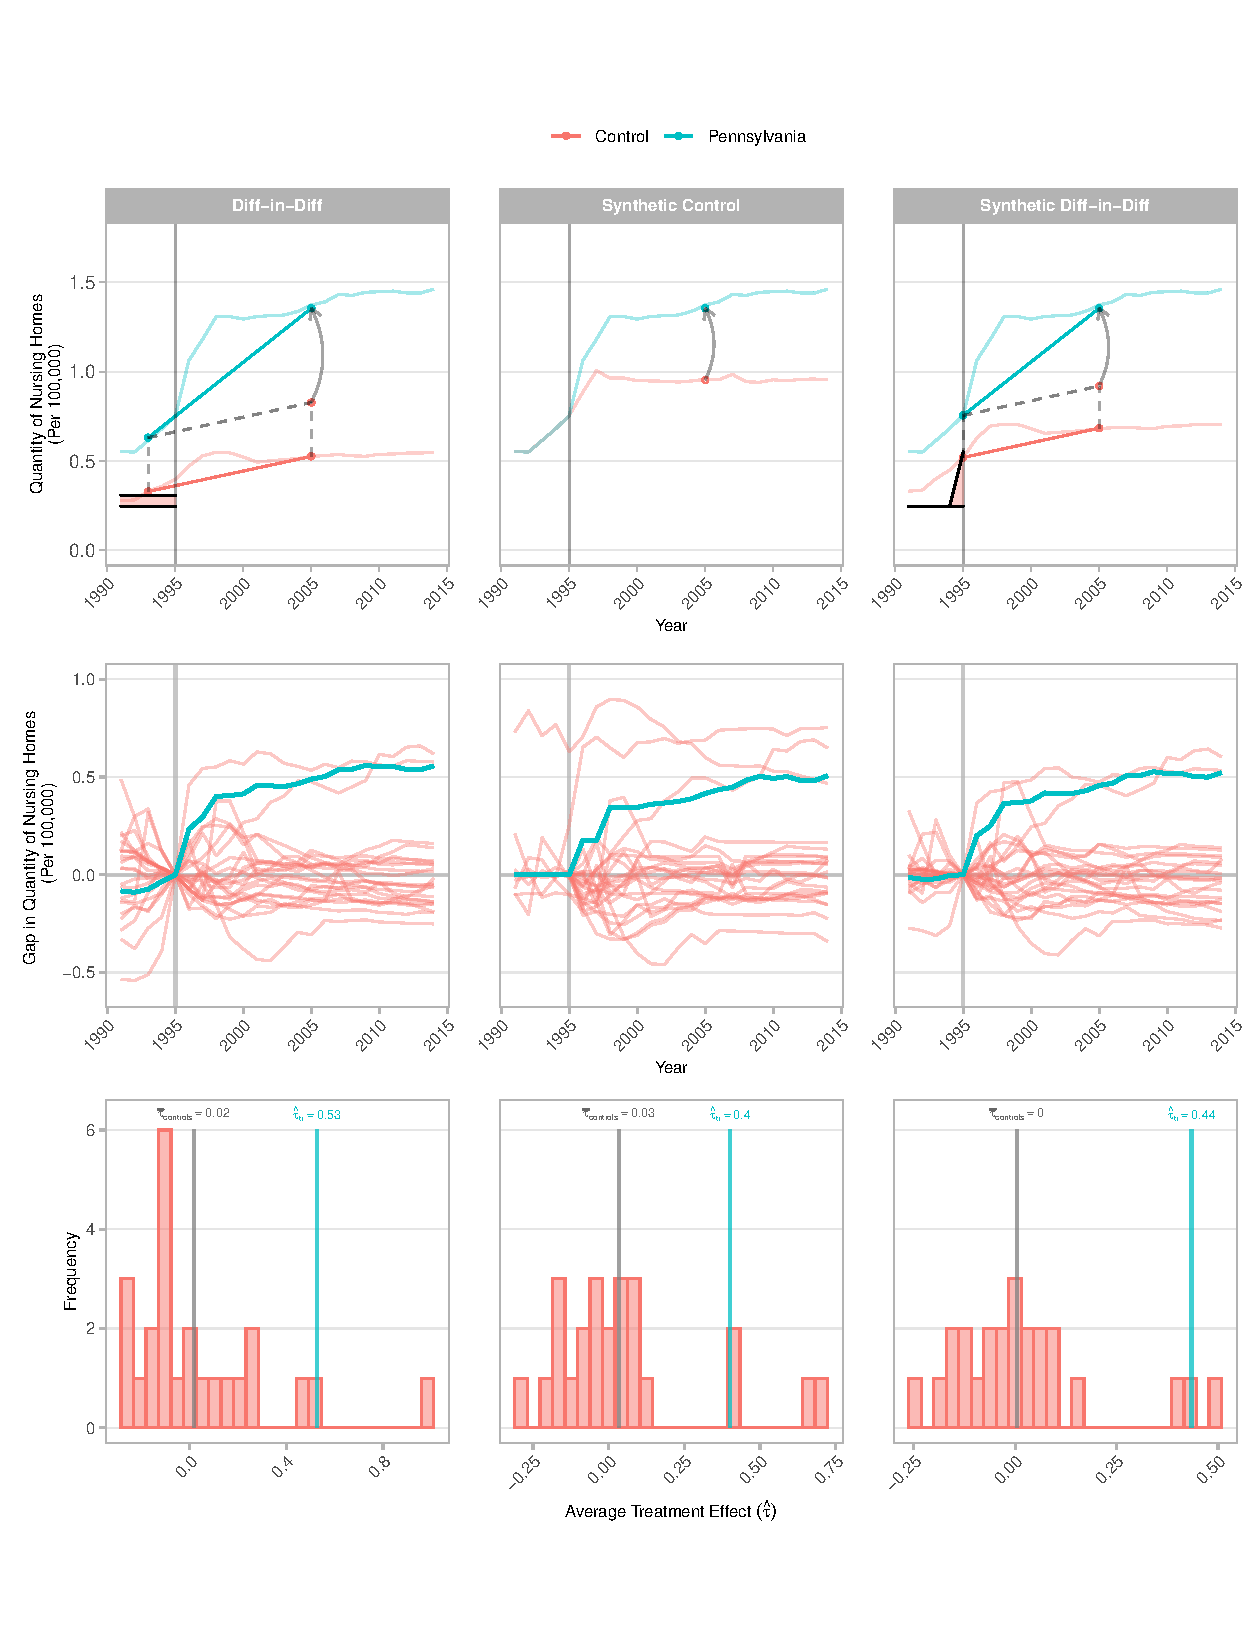
\includegraphics[width=\textwidth,keepaspectratio]{SynthDID_NoBord_NoCov/q_nh_plots_PA.pdf}}
    \vspace{-1.4cm}\\
    \scriptsize
		\textit{Notes}: The plots in the first row show trends in the quantity of nursing homes per 100,000 over time for Pennsylvania and for the relevant weighted average of control states, with the weights used to average pre-treatment time periods at the bottom of the plots. The curved arrows in the first row indicate the estimated average treatment effect, $\hat{\tau}$ from equation (\ref{eq:ave_effect_deltas}), and the vertical lines represent the year prior to PA dropping nursing home CON regulations. The plots in the second row show the year-specific difference in the quantity of nursing homes per 100,000 between PA and its corresponding weighted average of control states. The blue line shows these gaps for PA, and the pink lines show these gaps for each of the placebo control states used in the placebo variance estimation procedure outlined in Algorithm \ref{alg:two}. We make the gaps in the Diff-in-Diff and Synthetic Diff-in-Diff plots relative to their value in the year prior to PA dropping nursing home CON regulations (as indicated by the vertical lines). The plots in the third row show the distribution of placebo estimates ($\hat{\tau}^{(b)}$ from Algorithm \ref{alg:two}), with the mean of the placebo estimates and the actual estimated effect for PA indicated by the gray and blue vertical lines, respectively. Data source: 1991-2014 Centers for Medicare and Medicaid Services’ (CMS) Provider of Services files.
\end{figure}
\restoregeometry
\clearpage


%%%%%%%%%%% Quantity of Nursing Homes Per Capita - IN %%%%%%%%%%%
\newpage
\newgeometry{top=2cm}
%\setlength\abovecaptionskip{-1.5\baselineskip}
\begin{figure}[t] 
    \setlength\abovecaptionskip{-2\baselineskip}
	\caption{\label{fig:q_nh_plots_in} \centering A Comparison Between DID, SC, and SDID Estimates and Placebo Analysis for the Effect of Dropping Nursing Home CON Regulations on the Quantity of Nursing Homes Per 100,000 in Indiana} {\centering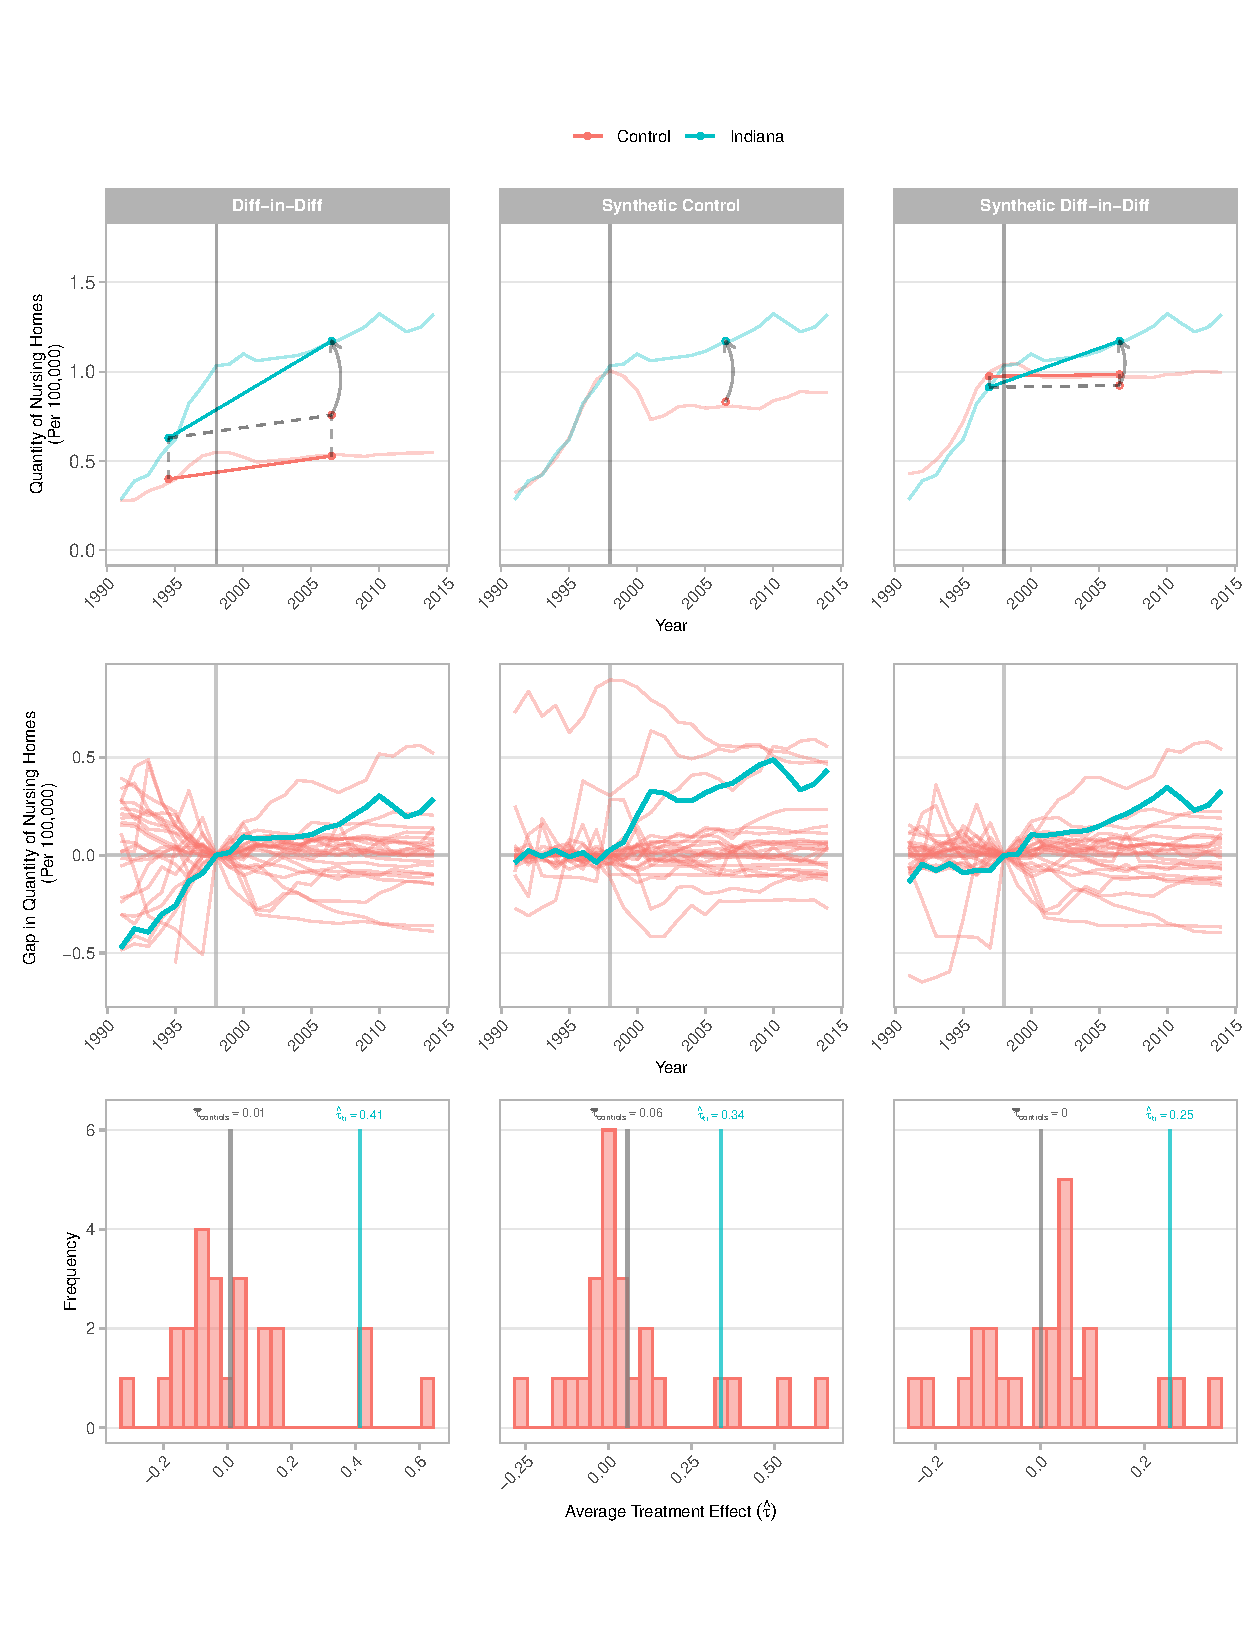
\includegraphics[width=\textwidth,keepaspectratio]{SynthDID_NoBord_NoCov/q_nh_plots_IN.pdf}}
    \vspace{-1.4cm}\\
    \scriptsize
		\textit{Notes}: The plots in the first row show trends in the quantity of nursing homes per 100,000 over time for Indiana and for the relevant weighted average of control states, with the weights used to average pre-treatment time periods at the bottom of the plots. The curved arrows in the first row indicate the estimated average treatment effect, $\hat{\tau}$ from equation (\ref{eq:ave_effect_deltas}), and the vertical lines represent the year prior to IN dropping nursing home CON regulations. The plots in the second row show the year-specific difference in the quantity of nursing homes per 100,000 between IN and its corresponding weighted average of control states. The blue line shows these gaps for IN, and the pink lines show these gaps for each of the placebo control states used in the placebo variance estimation procedure outlined in Algorithm \ref{alg:two}. We make the gaps in the Diff-in-Diff and Synthetic Diff-in-Diff plots relative to their value in the year prior to IN dropping nursing home CON regulations (as indicated by the vertical lines). The plots in the third row show the distribution of placebo estimates ($\hat{\tau}^{(b)}$ from Algorithm \ref{alg:two}), with the mean of the placebo estimates and the actual estimated effect for IN indicated by the gray and blue vertical lines, respectively. Data source: 1991-2014 Centers for Medicare and Medicaid Services’ (CMS) Provider of Services files.
\end{figure}
\restoregeometry
\clearpage


%%%%%%%%%%% Quantity of Nursing Homes Per Capita - ND %%%%%%%%%%%
\newpage
\newgeometry{top=2cm}
%\setlength\abovecaptionskip{-1.5\baselineskip}
\begin{figure}[t] 
    \setlength\abovecaptionskip{-2\baselineskip}
	\caption{\label{fig:q_nh_plots_nd} \centering A Comparison Between DID, SC, and SDID Estimates and Placebo Analysis for the Effect of Dropping Nursing Home CON Regulations on the Quantity of Nursing Homes Per 100,000 in North Dakota} {\centering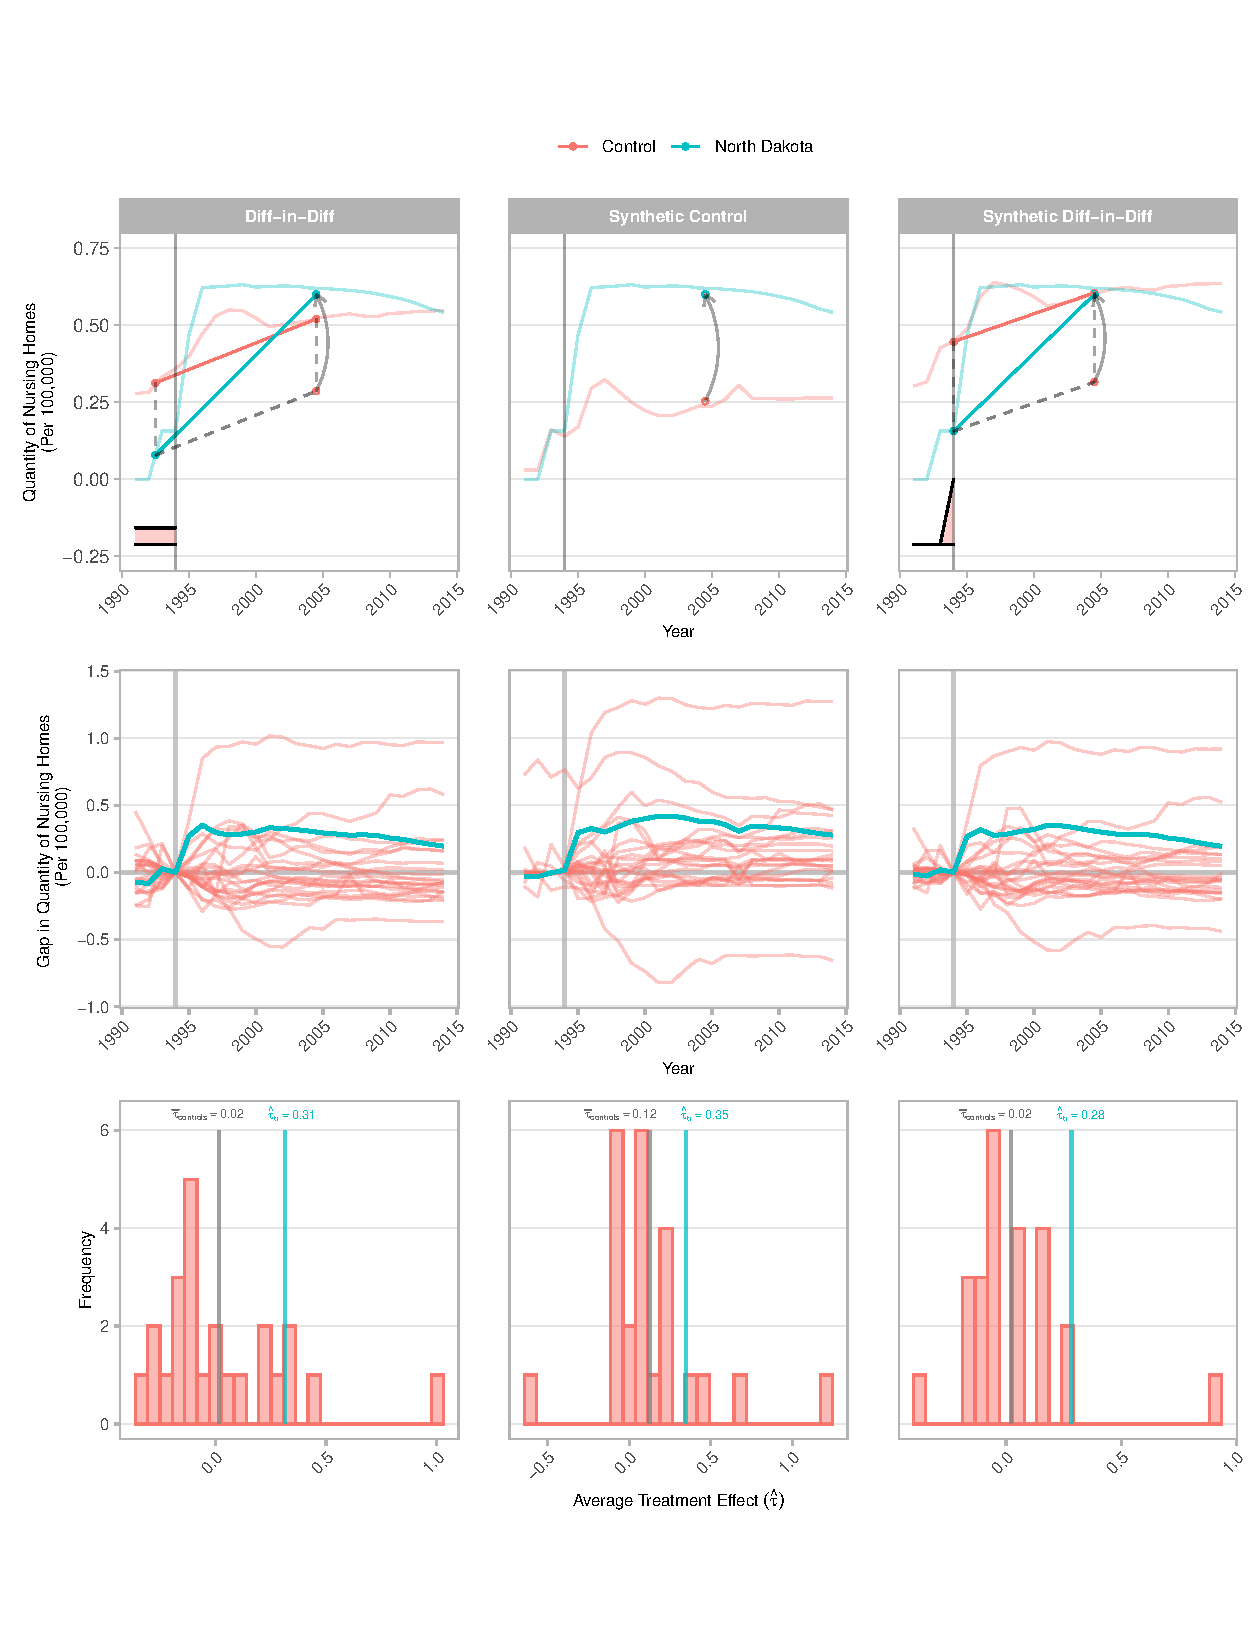
\includegraphics[width=\textwidth,keepaspectratio]{SynthDID_NoBord_NoCov/q_nh_plots_ND.pdf}}
    \vspace{-1.4cm}\\
    \scriptsize
		\textit{Notes}: The plots in the first row show trends in the quantity of nursing homes per 100,000 over time for North Dakota and for the relevant weighted average of control states, with the weights used to average pre-treatment time periods at the bottom of the plots. The curved arrows in the first row indicate the estimated average treatment effect, $\hat{\tau}$ from equation (\ref{eq:ave_effect_deltas}), and the vertical lines represent the year prior to ND dropping nursing home CON regulations. The plots in the second row show the year-specific difference in the quantity of nursing homes per 100,000 between ND and its corresponding weighted average of control states. The blue line shows these gaps for ND, and the pink lines show these gaps for each of the placebo control states used in the placebo variance estimation procedure outlined in Algorithm \ref{alg:two}. We make the gaps in the Diff-in-Diff and Synthetic Diff-in-Diff plots relative to their value in the year prior to ND dropping nursing home CON regulations (as indicated by the vertical lines). The plots in the third row show the distribution of placebo estimates ($\hat{\tau}^{(b)}$ from Algorithm \ref{alg:two}), with the mean of the placebo estimates and the actual estimated effect for ND indicated by the gray and blue vertical lines, respectively. Data source: 1991-2014 Centers for Medicare and Medicaid Services’ (CMS) Provider of Services files.
\end{figure}
\restoregeometry
\clearpage


%%%%%%%%% Quantity of Specialized Beds Per 100,000 - PA %%%%%%%%%
\newpage
\newgeometry{top=2cm}
%\setlength\abovecaptionskip{-1.5\baselineskip}
\begin{figure}[t] 
    \setlength\abovecaptionskip{-2\baselineskip}
	\caption{\label{fig:q_specbeds_plots_pa} \centering A Comparison Between DID, SC, and SDID Estimates and Placebo Analysis for the Effect of Dropping Nursing Home CON Regulations on the Quantity of Specialized Nursing Home Beds Per 100,000 in Pennsylvania} {\centering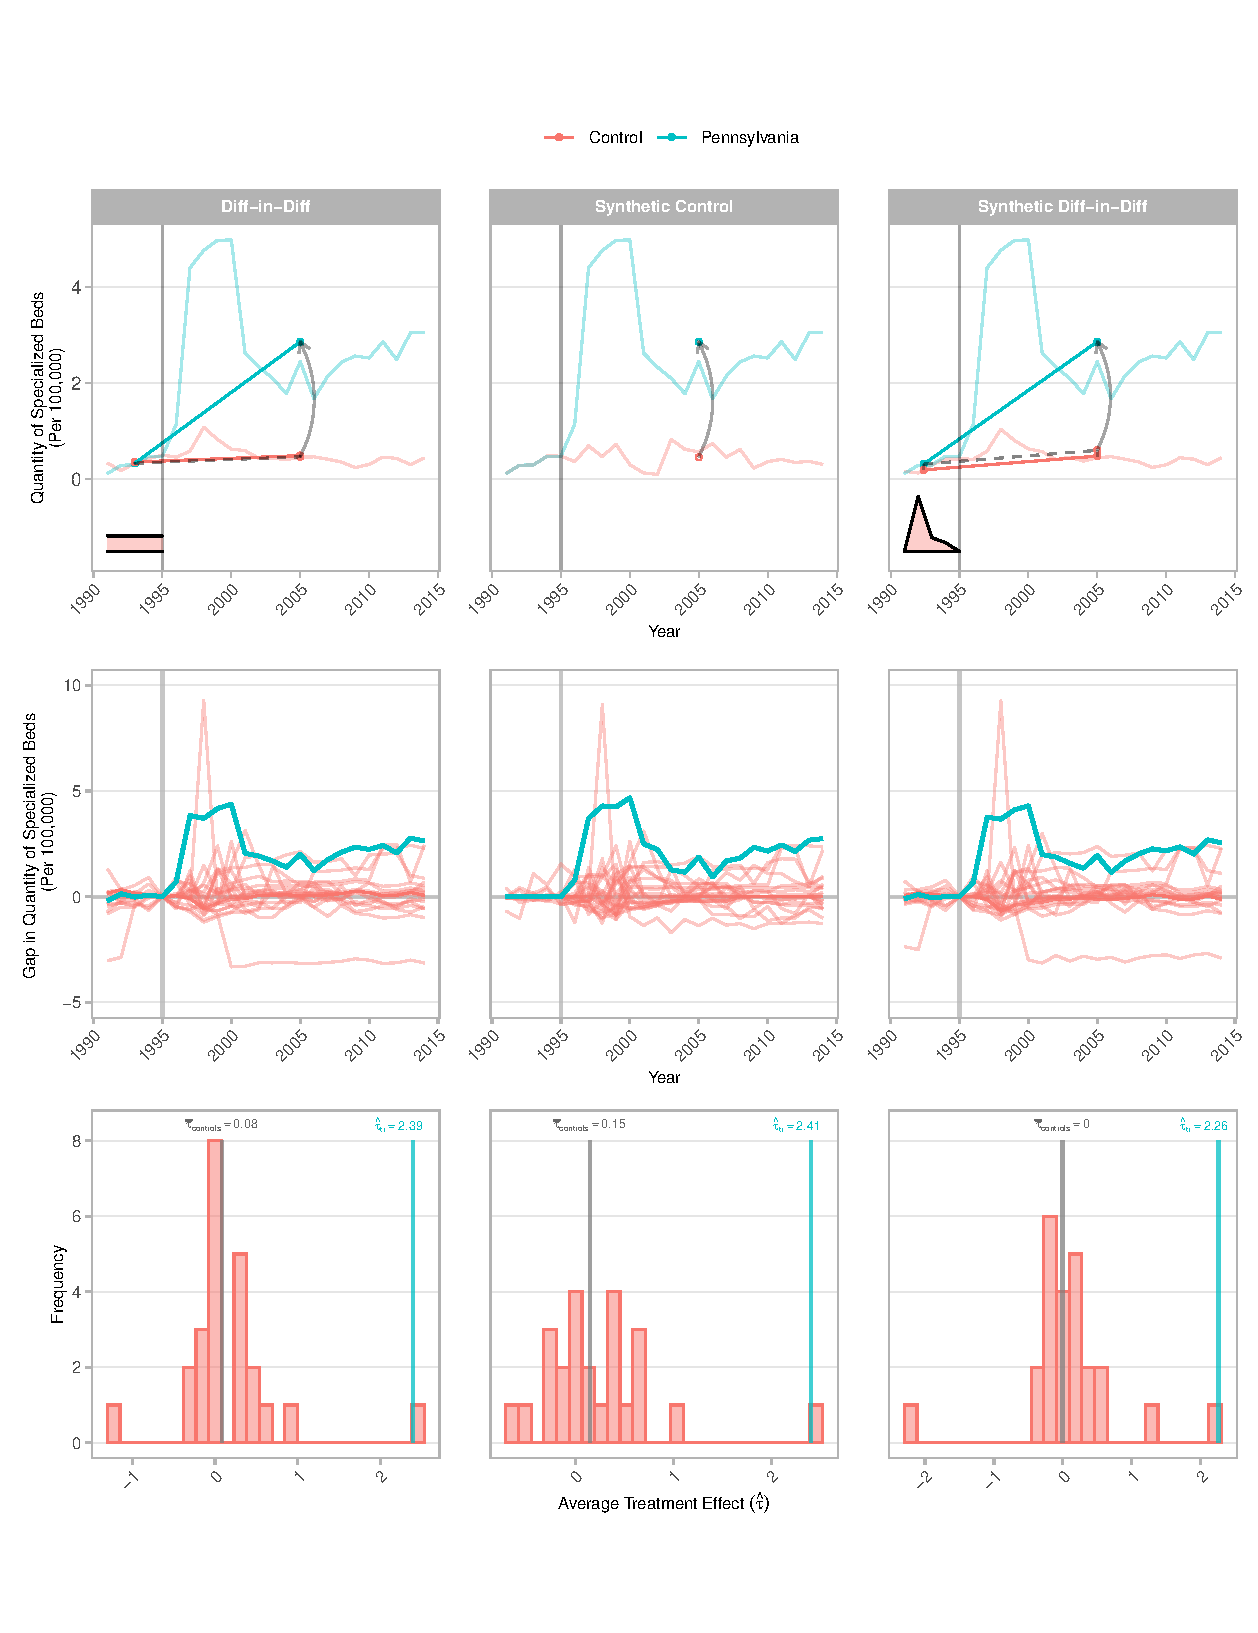
\includegraphics[width=\textwidth,keepaspectratio]{SynthDID_NoBord_NoCov/q_specbeds_plots_PA.pdf}}
    \vspace{-1.4cm}\\
    \scriptsize
		\textit{Notes}: The plots in the first row show trends in the quantity of specialized nursing home beds per 100,000 over time for Pennsylvania and for the relevant weighted average of control states, with the weights used to average pre-treatment time periods at the bottom of the plots. The curved arrows in the first row indicate the estimated average treatment effect, $\hat{\tau}$ from equation (\ref{eq:ave_effect_deltas}), and the vertical lines represent the year prior to PA dropping nursing home CON regulations. The plots in the second row show the year-specific difference in the quantity of specialized nursing home beds per 100,000 between PA and its corresponding weighted average of control states. The blue line shows these gaps for PA, and the pink lines show these gaps for each of the placebo control states used in the placebo variance estimation procedure outlined in Algorithm \ref{alg:two}. We make the gaps in the Diff-in-Diff and Synthetic Diff-in-Diff plots relative to their value in the year prior to PA dropping nursing home CON regulations (as indicated by the vertical lines). The plots in the third row show the distribution of placebo estimates ($\hat{\tau}^{(b)}$ from Algorithm \ref{alg:two}), with the mean of the placebo estimates and the actual estimated effect for PA indicated by the gray and blue vertical lines, respectively. Data source: 1991-2014 Centers for Medicare and Medicaid Services’ (CMS) Provider of Services files.
\end{figure}
\restoregeometry
\clearpage


%%%%%%%%% Quantity of Specialized Beds Per 100,000 - IN %%%%%%%%%
\newpage
\newgeometry{top=2cm}
%\setlength\abovecaptionskip{-1.5\baselineskip}
\begin{figure}[t] 
    \setlength\abovecaptionskip{-2\baselineskip}
	\caption{\label{fig:q_specbeds_plots_in} \centering A Comparison Between DID, SC, and SDID Estimates and Placebo Analysis for the Effect of Dropping Nursing Home CON Regulations on the Quantity of Specialized Nursing Home Beds Per 100,000 in Indiana} {\centering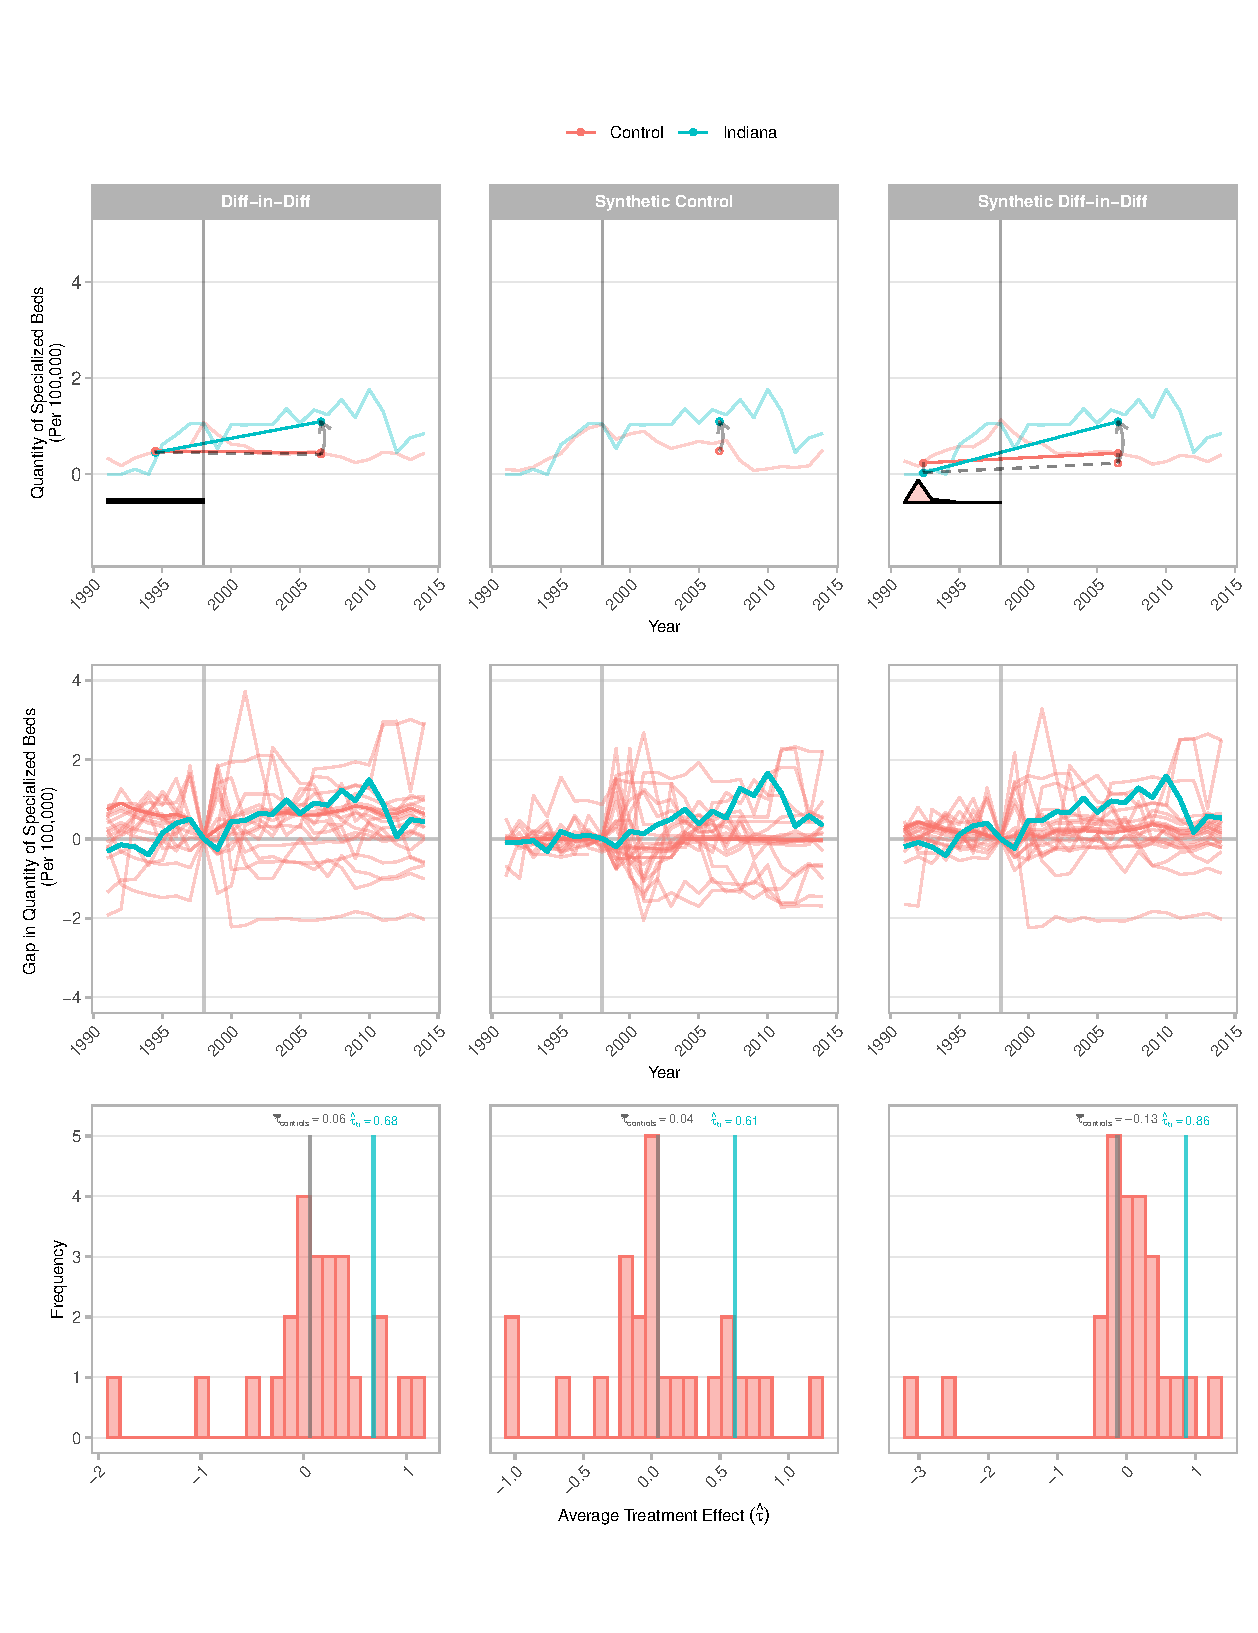
\includegraphics[width=\textwidth,keepaspectratio]{SynthDID_NoBord_NoCov/q_specbeds_plots_IN.pdf}}
    \vspace{-1.4cm}\\
    \scriptsize
		\textit{Notes}: The plots in the first row show trends in the quantity of specialized nursing home beds per 100,000 over time for Indiana and for the relevant weighted average of control states, with the weights used to average pre-treatment time periods at the bottom of the plots. The curved arrows in the first row indicate the estimated average treatment effect, $\hat{\tau}$ from equation (\ref{eq:ave_effect_deltas}), and the vertical lines represent the year prior to IN dropping nursing home CON regulations. The plots in the second row show the year-specific difference in the quantity of specialized nursing home beds per 100,000 between IN and its corresponding weighted average of control states. The blue line shows these gaps for IN, and the pink lines show these gaps for each of the placebo control states used in the placebo variance estimation procedure outlined in Algorithm \ref{alg:two}. We make the gaps in the Diff-in-Diff and Synthetic Diff-in-Diff plots relative to their value in the year prior to IN dropping nursing home CON regulations (as indicated by the vertical lines). The plots in the third row show the distribution of placebo estimates ($\hat{\tau}^{(b)}$ from Algorithm \ref{alg:two}), with the mean of the placebo estimates and the actual estimated effect for IN indicated by the gray and blue vertical lines, respectively. Data source: 1991-2014 Centers for Medicare and Medicaid Services’ (CMS) Provider of Services files.
\end{figure}
\restoregeometry
\clearpage

\begin{comment}
%%%%%%%%% Quantity of Specialized Beds Per 100,000 - ND %%%%%%%%%
\newpage
\newgeometry{top=2cm}
%\setlength\abovecaptionskip{-1.5\baselineskip}
\begin{figure}[t] 
    \setlength\abovecaptionskip{-2\baselineskip}
	\caption{\label{fig:q_specbeds_plots_nd} \centering A Comparison Between DID, SC, and SDID Estimates and Placebo Analysis for the Effect of Dropping Nursing Home CON Regulations on the Quantity of Specialized Nursing Home Beds Per 100,000 in North Dakota} {\centering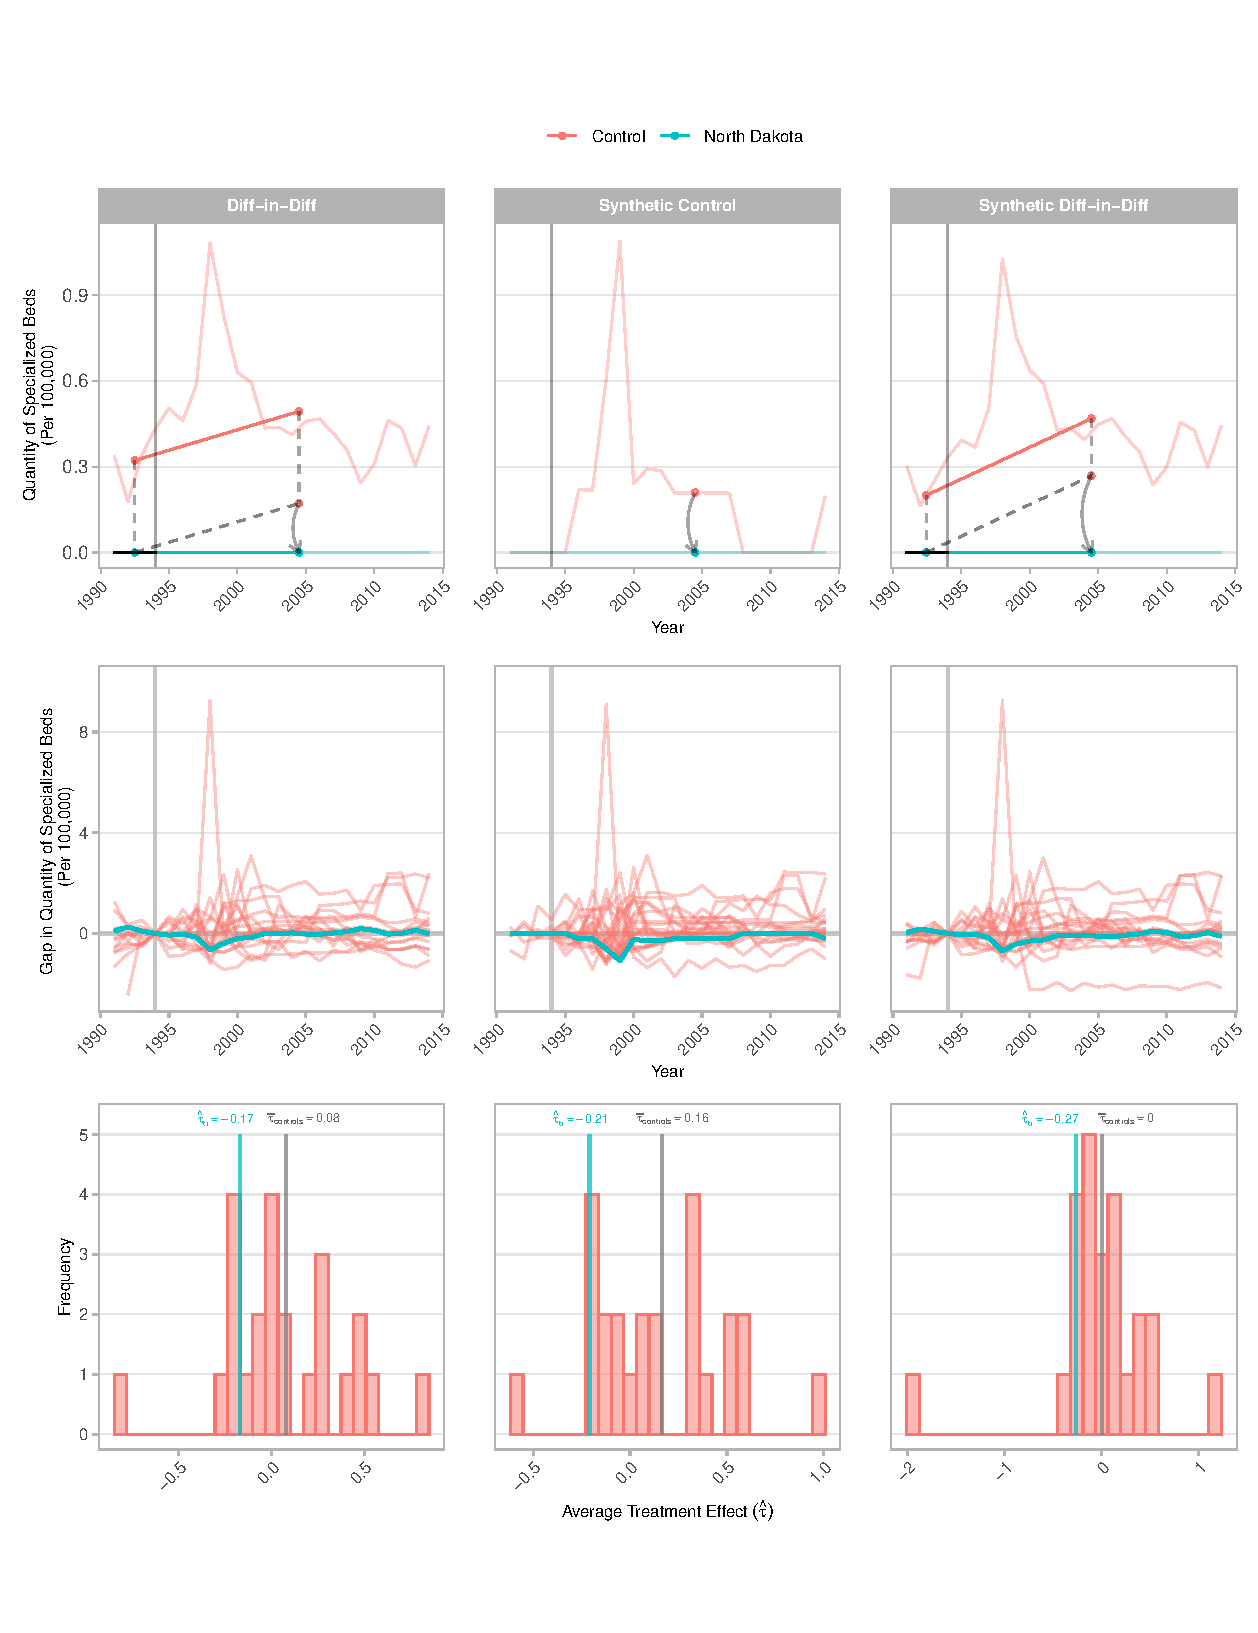
\includegraphics[width=\textwidth,keepaspectratio]{SynthDID_NoBord_NoCov/q_specbeds_plots_ND.pdf}}
    \vspace{-1.4cm}\\
    \scriptsize
		\textit{Notes}: The plots in the first row show trends in the quantity of specialized nursing home beds per 100,000 over time for North Dakota and for the relevant weighted average of control states, with the weights used to average pre-treatment time periods at the bottom of the plots. The curved arrows in the first row indicate the estimated average treatment effect, $\hat{\tau}$ from equation (\ref{eq:ave_effect_deltas}), and the vertical lines represent the year prior to ND dropping nursing home CON regulations. The plots in the second row show the year-specific difference in the quantity of specialized nursing home beds per 100,000 between ND and its corresponding weighted average of control states. The blue line shows these gaps for ND, and the pink lines show these gaps for each of the placebo control states used in the placebo variance estimation procedure outlined in Algorithm \ref{alg:two}. We make the gaps in the Diff-in-Diff and Synthetic Diff-in-Diff plots relative to their value in the year prior to ND dropping nursing home CON regulations (as indicated by the vertical lines). The plots in the third row show the distribution of placebo estimates ($\hat{\tau}^{(b)}$ from Algorithm \ref{alg:two}), with the mean of the placebo estimates and the actual estimated effect for ND indicated by the gray and blue vertical lines, respectively. Data source: 1991-2014 Centers for Medicare and Medicaid Services’ (CMS) Provider of Services files.
\end{figure}
\restoregeometry
\clearpage
\end{comment}


\end{document}